% ---
% Arquivo com a execução do Trabalho de Conclusão de Curso dos alunos
% Gabriel Takaoka Nishimura, Felippe Demarqui Ramos e Vivian Kimie Isuyama 
% da Escola Politécnica da Universidade de São Paulo
% ---
	\chapter{Execução}\label{cap-execucao}
	
	\section{Arquitetura}
	
	\begin{figure}[htb]
		\caption{\label{fig_arch} Desenho esquemático}
		\centering
		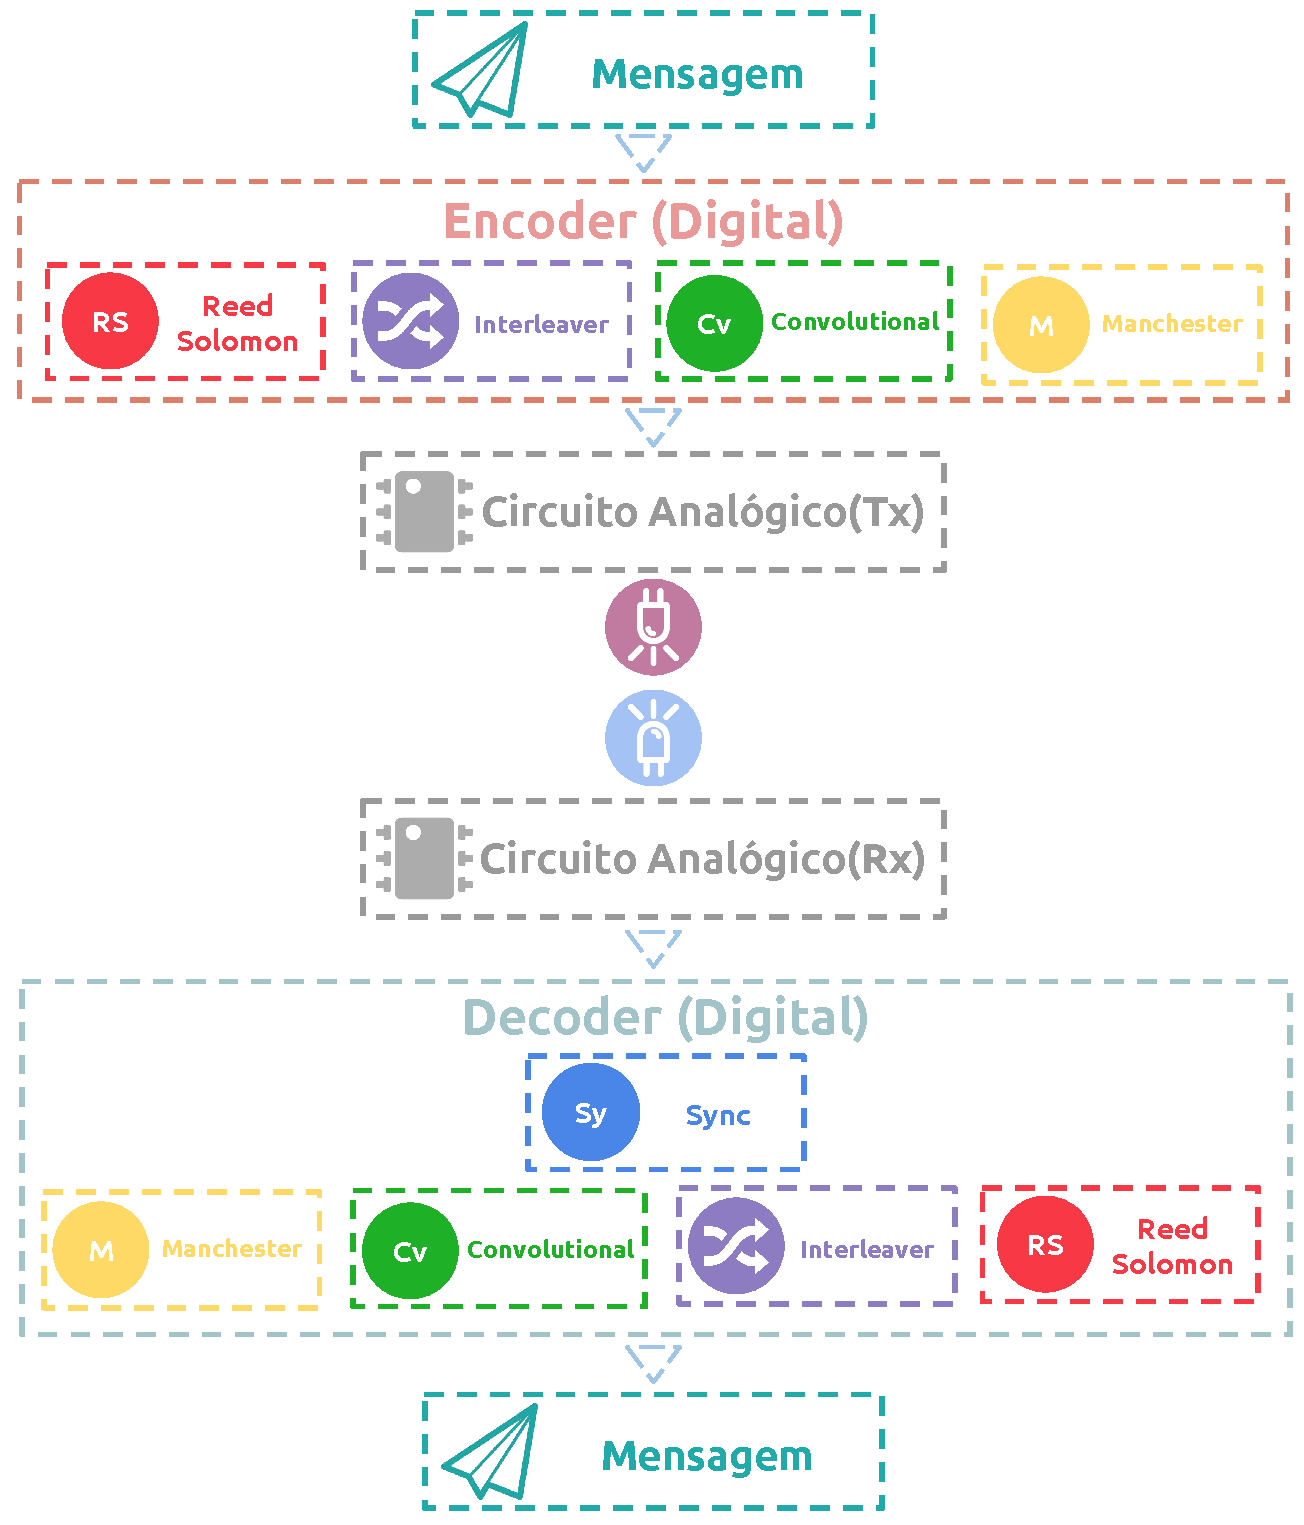
\includegraphics[width=1\textwidth]{Arquitetura}
		\legend{Fonte: Autores.}
	\end{figure}
	
	
	\subsection{Codificador}
	
	Conforme apontado no capítulo de Metodologia, a arquitetura do codificador Reed Solomon foi construída para um código (15, 7), portanto contando com 8 registradores em série. Os multiplicadores foram feitos com uma tabela,  que recebe duas entradas e retorna uma saída, de maneira a simplificar o trabalho de fazer uma função utilizando lógica combinatória. Já os somadores são equivalentes à função de OU exclusivo, ou XOR, com duas entradas e uma saída de 4 bits cada - ou seja, um símbolo. Além destes, os módulos básicos ainda compreendem um multiplexador, que seleciona um entre dois símbolos. A arquitetura desenvolvida pode ser observada na \autoref{RS_encoder_logic}.
	
	O comportamento de codificação de uma mensagem pode ser exemplificado pela \autoref{simula_rs_encoder}, onde se observa a entrada de uma mensagem de 7 símbolos e a saída de um bloco de 15 símbolos, sendo 8 de paridade.
	
	\begin{figure}[htb]
		\caption{\label{simula_rs_encoder} Simulação de codificação do codificador Reed Solomon}
		\centering
		\includegraphics[width=1\textwidth]{RS/Sim_encoder}
		\legend{Fonte: Autores.}
	\end{figure}
	
	\subsection{Decodificador}
	
	A arquitetura do decodificador segue o diagrama funcional da figura X do capítulo de Metologia. Desta forma, o desenvolvimento pode ser separado em quatro partes principais, apresentadas a seguir.
	
	\subsubsection{Cálculo das Síndromes}
	
	O cálculo das síndromes é feito de forma iterativa, durando tantos ciclos quanto forem os símbolos da mensagem. O cálculo de cada síndrome é independente dos cálculos das demais, e depende apenas dos símbolos de entrada e de cada uma das raízes do polinômio codificador, de alpha0 a alpha7 neste caso. O arranjo dos componentes pode se exemplificar através da arquitetura do módulo, representada a seguir.
	
	\begin{figure}[!htb]
		\caption{\label{fig_sindrome_arq} Arquitetura do módulo de cálculo das síndromes}
		\centering
		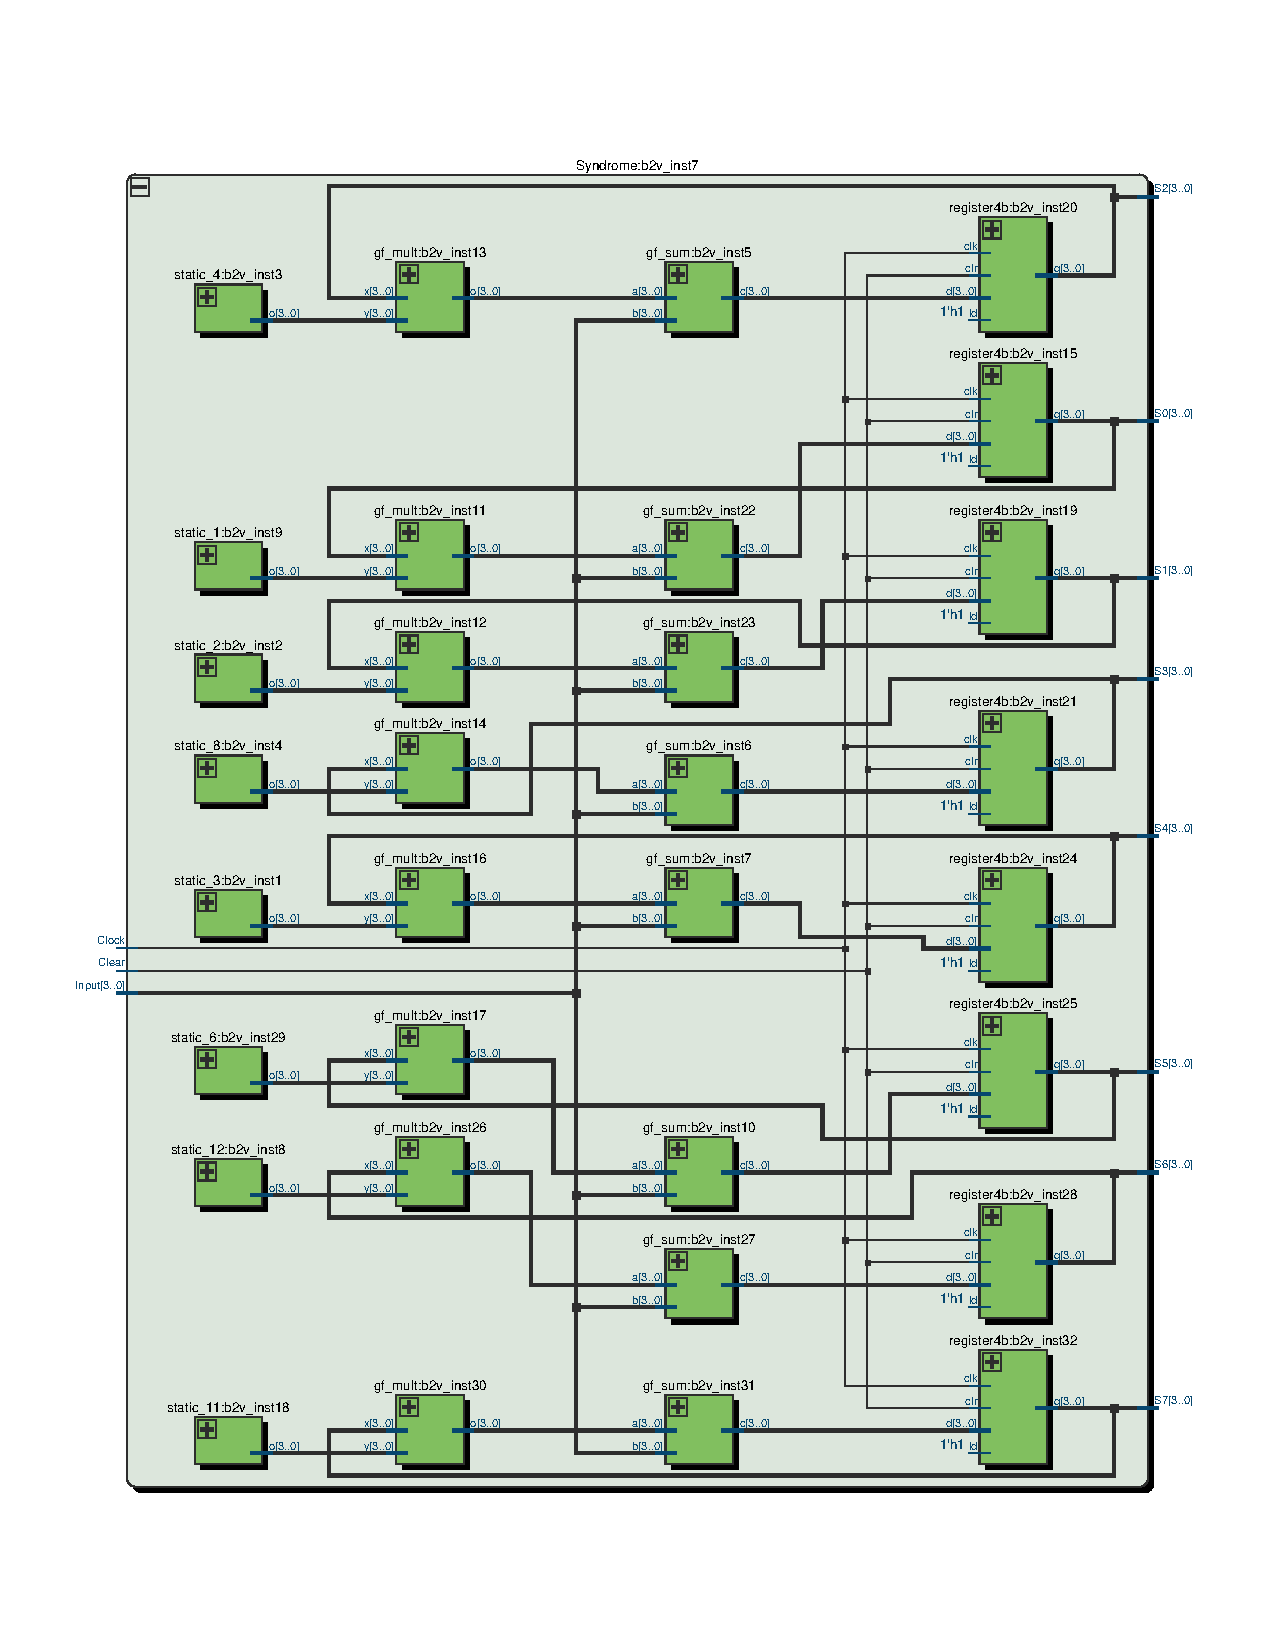
\includegraphics[width=1\textwidth]{RS/SindromeRTL.pdf}
		\legend{}
	\end{figure}
	
	
	Os elementos indicados por "static" são constantes, guardando os valores dos símbolos de cada umas raízes citadas. Estes valores são enviados para multiplicadores de GF(16), representados por "gfmult". Como pode-se observar, o cálculo é iterativo e portanto os multiplicadores recebem também o valor dos registradores que são representados por "register4b". Os somadores de Campos de Galois são representados por "gfsum".
	
	A simulação a seguir representa o caso em que existem erros na mensagem codificada, o que é indicado por síndromes diferentes de 0000.
	
	\begin{figure}[!htb]
		\caption{\label{fig_sindrome_sim} Simulação do cálculo das síndromes}
		\centering
		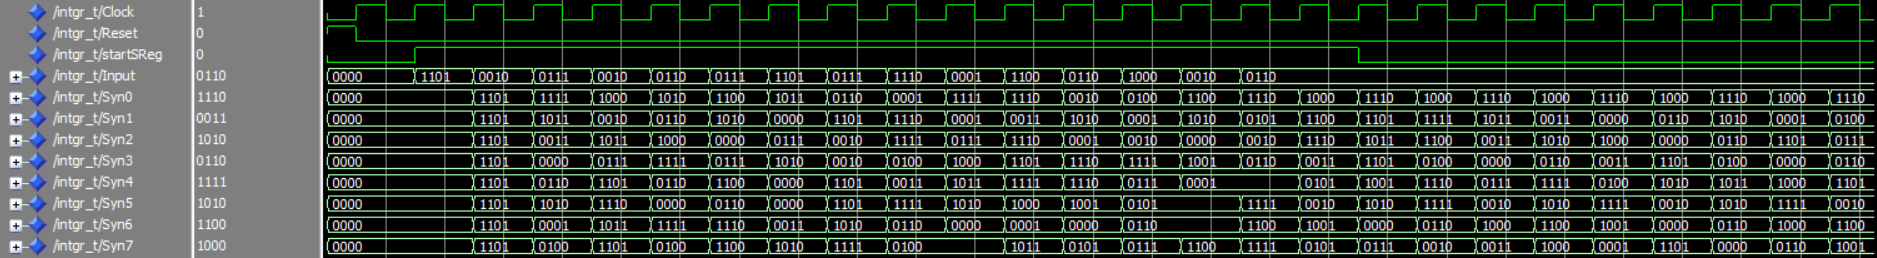
\includegraphics[width=1\textwidth]{RS/Sim_sindrome.PNG}
		\legend{}
	\end{figure}

	\subsubsection{Módulo de Berlekamp-Massey}
	
	O módulo de Berlekamp-Massey foi implementado de forma a primeiramente calcular as localizações dos erros, ou seja, os coeficientes do polinômio localizador de erros, representados por Lamba, e guardados em registradores, para o posterior cálculo dos valores dos erros. Os valores de erros são calculados então, com as síndromes e localizações de erro.
	
	\begin{figure}[!htb]
		\caption{\label{fig_berlekamp_arq} Arquitetura do módulo de Berlekamp-Massey}
		\centering
		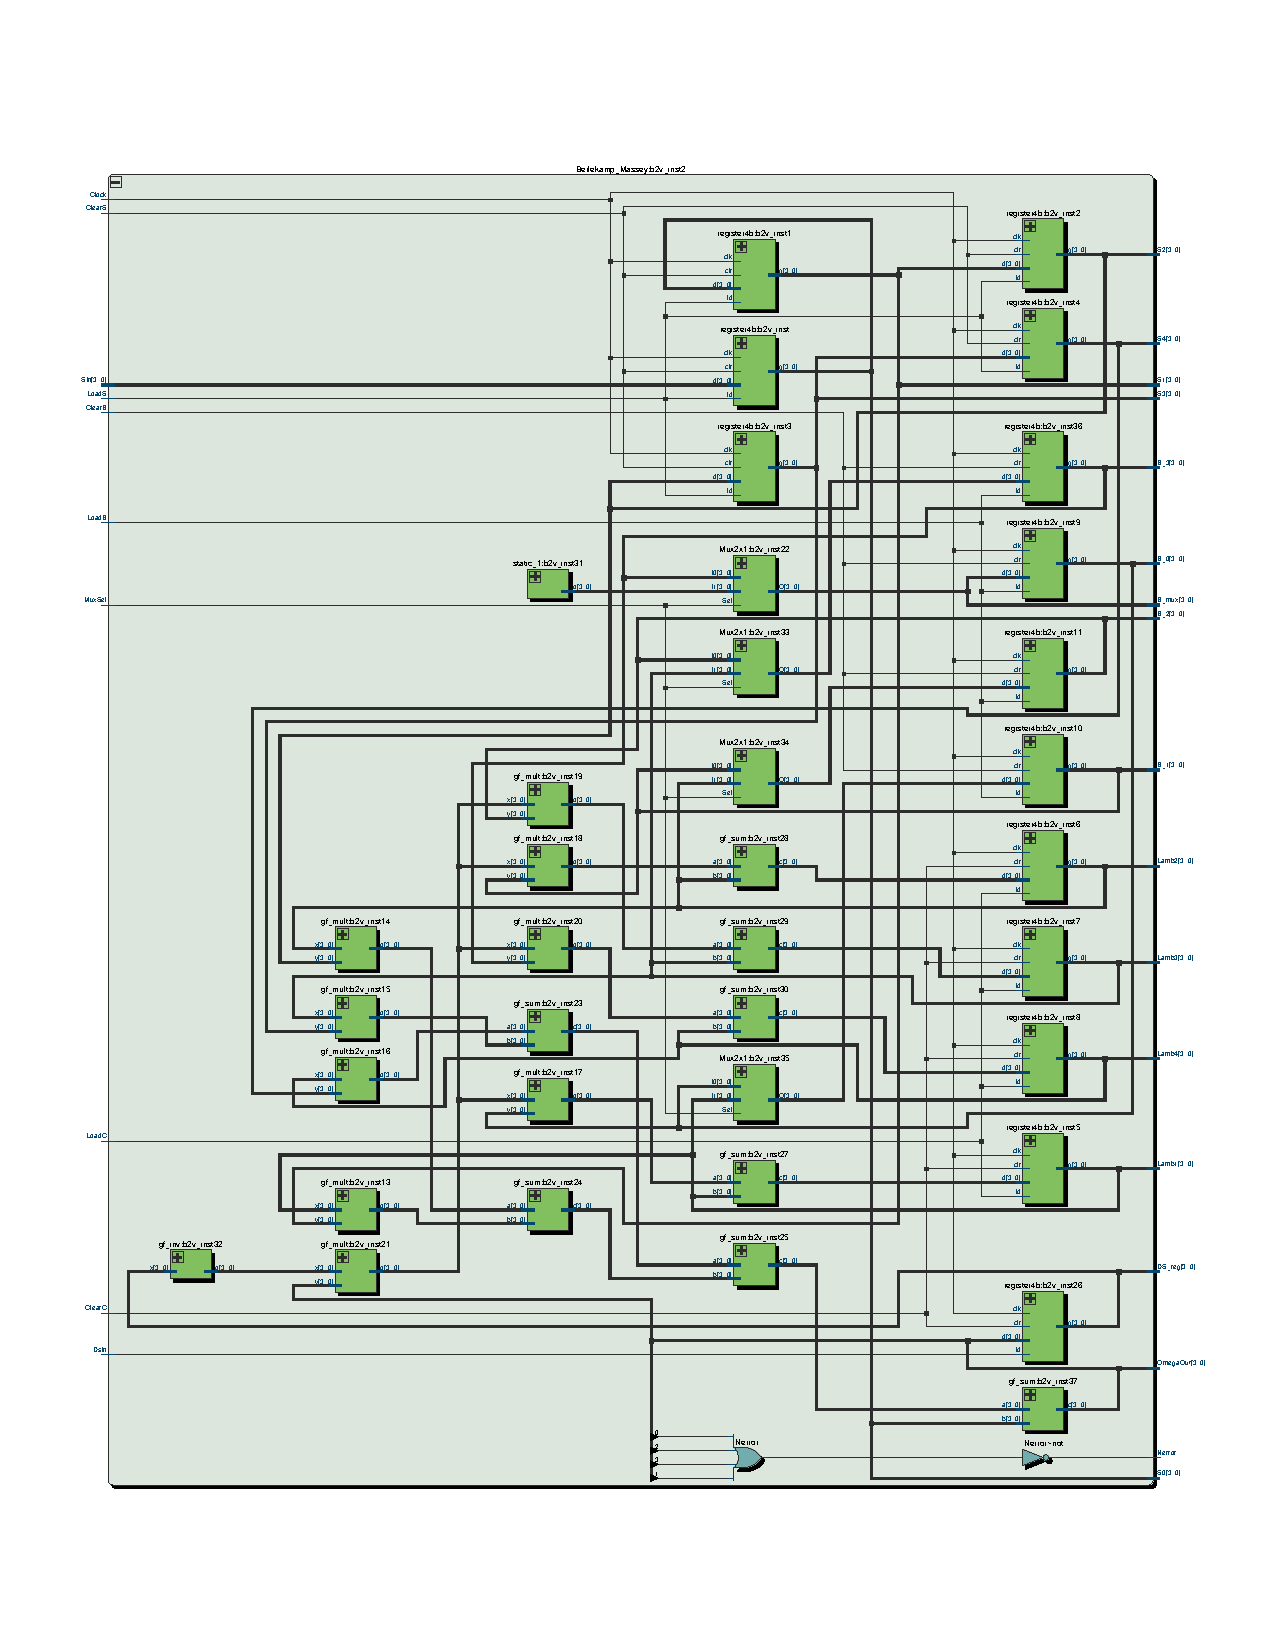
\includegraphics[width=1\textwidth]{RS/BerlekampRTL.pdf}
		\legend{}
	\end{figure}
	
	As síndromes são enviadas sequencialmente para o módulo de Berlekamp-Massey a cada ciclo de clock. A atualização do polinômio localizador, representado pela seção X do diagrama, ocorre quando ele não possibilitar gerar uma síndrome específica. Nesse caso, são feitos os cálculos no módulo inversor, com a atualização do polinômio no próximo ciclo. Esse processo é exemplificado pela \autoref{fig_berlekamp_sim}.
	
	\begin{figure}[!htb]
		\caption{\label{fig_berlekamp_sim} Simulação do módulo de Berlekamp-Massey}
		\centering
		\includegraphics[width=1\textwidth]{RS/Sim_berlekamp.PNG}
		\legend{}
	\end{figure}
	
	Uma vez calculados os valores dos coeficientes do polinômio localizador, equivalentes a Lambda na simulação, é necessário calcular os coeficientes do polinômio de valor dos erros. Novamente, as síndromes são enviadas sequencialmente para o circuito. O novo cálculo ocorre com as síndromes e o polinômio localizador de erros. O resultado são os coeficientes do polinômio de valores de erro, representados por Omega na simulação, obtidos em sequência em cada ciclo de clock. 
	
	O componente de Berlekamp-Massey possui um circuito de controle próprio. Por ele é recebido um sinal de início de cálculo, vindo do controlador do estágio anterior, de cálculo de síndromes. Sendo assim, ele deve manipular registradores, para, por exemplo, registrar os valores de Lambda e Omega para cálculo posterior, no módulo seguinte.
	
	\subsubsection{Módulos de Busca de Chien e Forney}
	
	O módulo de busca de Chien é na verdade composto por dois módulos: busca de localização e de valores dos erros. Ambos trabalham paralelamente e têm como entrada os coeficientes $\Lambda$ e $\Omega$. 
	
	\begin{figure}[!htb]
		\caption{\label{fig_chienloc_arq} Arquitetura do módulo de busca de Chien: localização de erros}
		\centering
		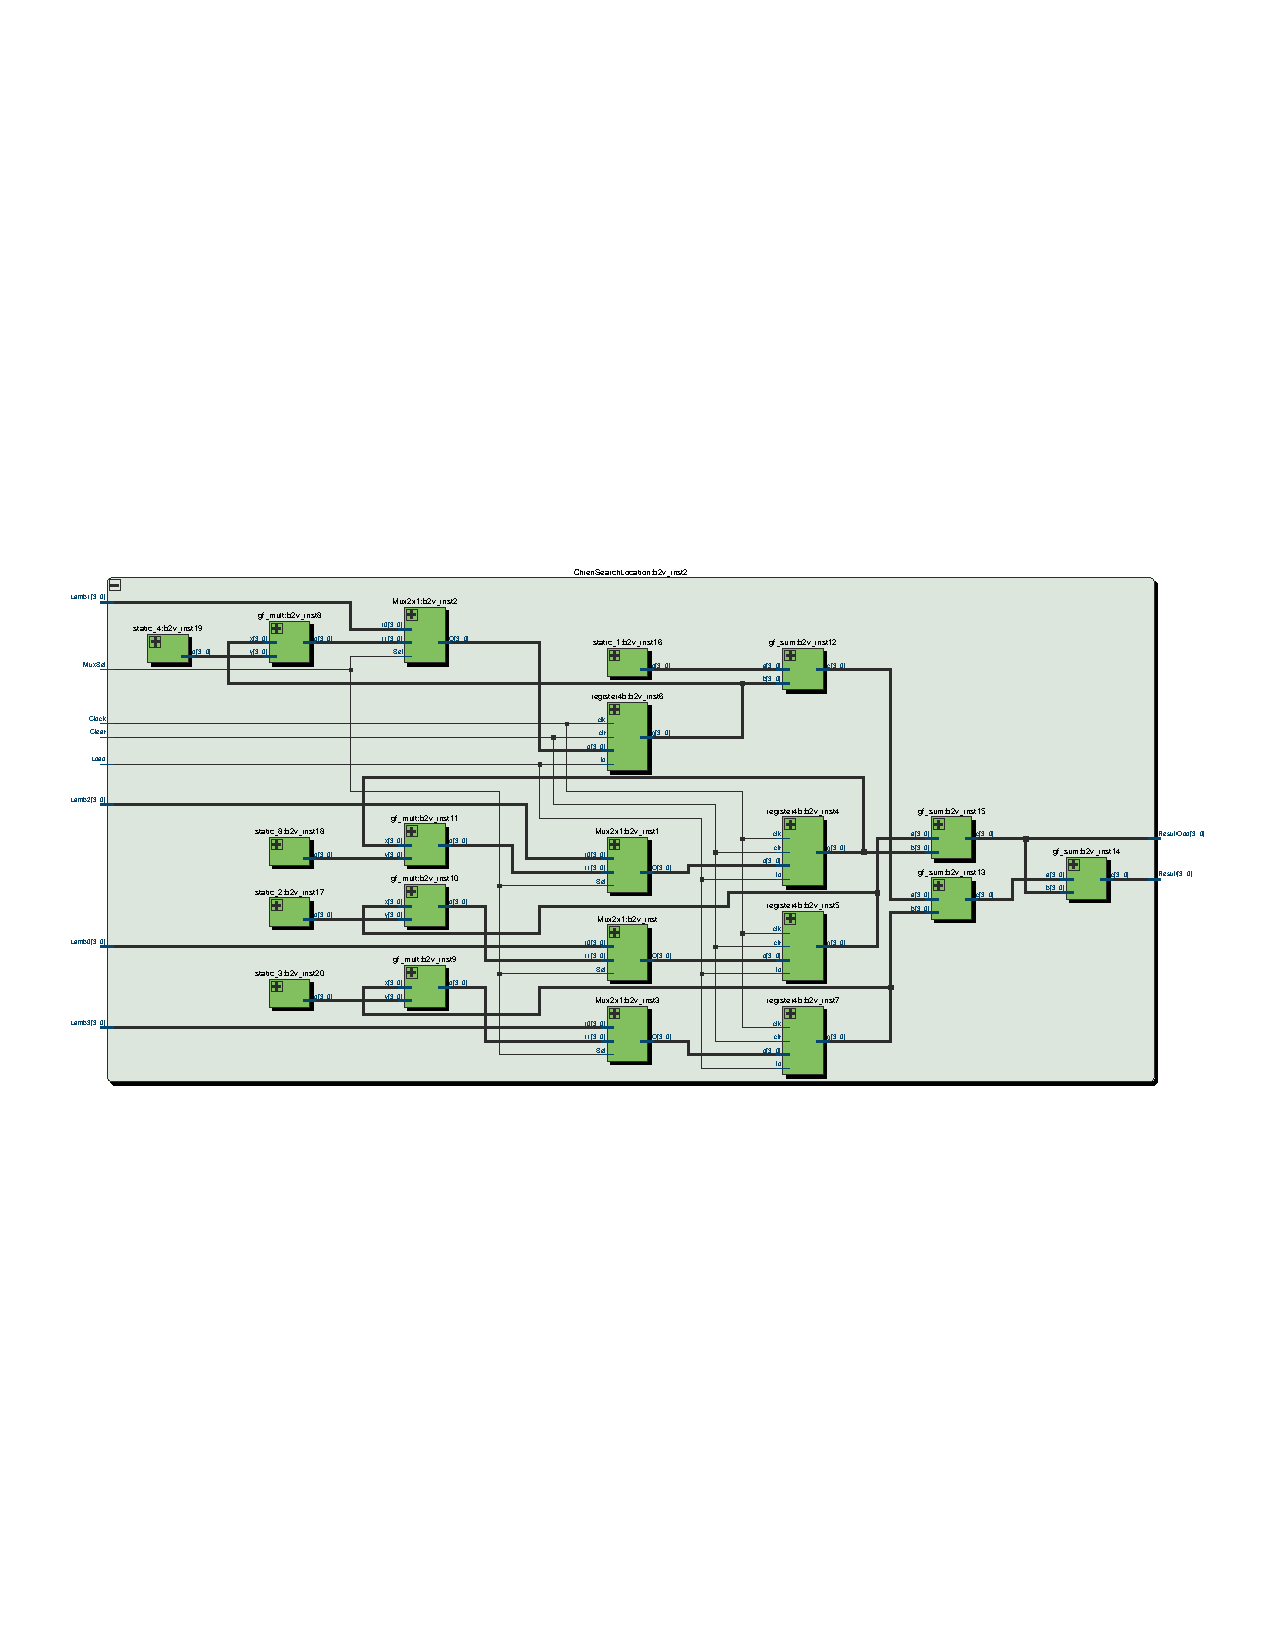
\includegraphics[width=1\textwidth]{RS/ChienLocationRTL.pdf}
		\legend{}
	\end{figure}

	\begin{figure}[!htb]
		\caption{\label{fig_chienval_arq} Arquitetura do módulo de busca de Chien: valores de erros}
		\centering
		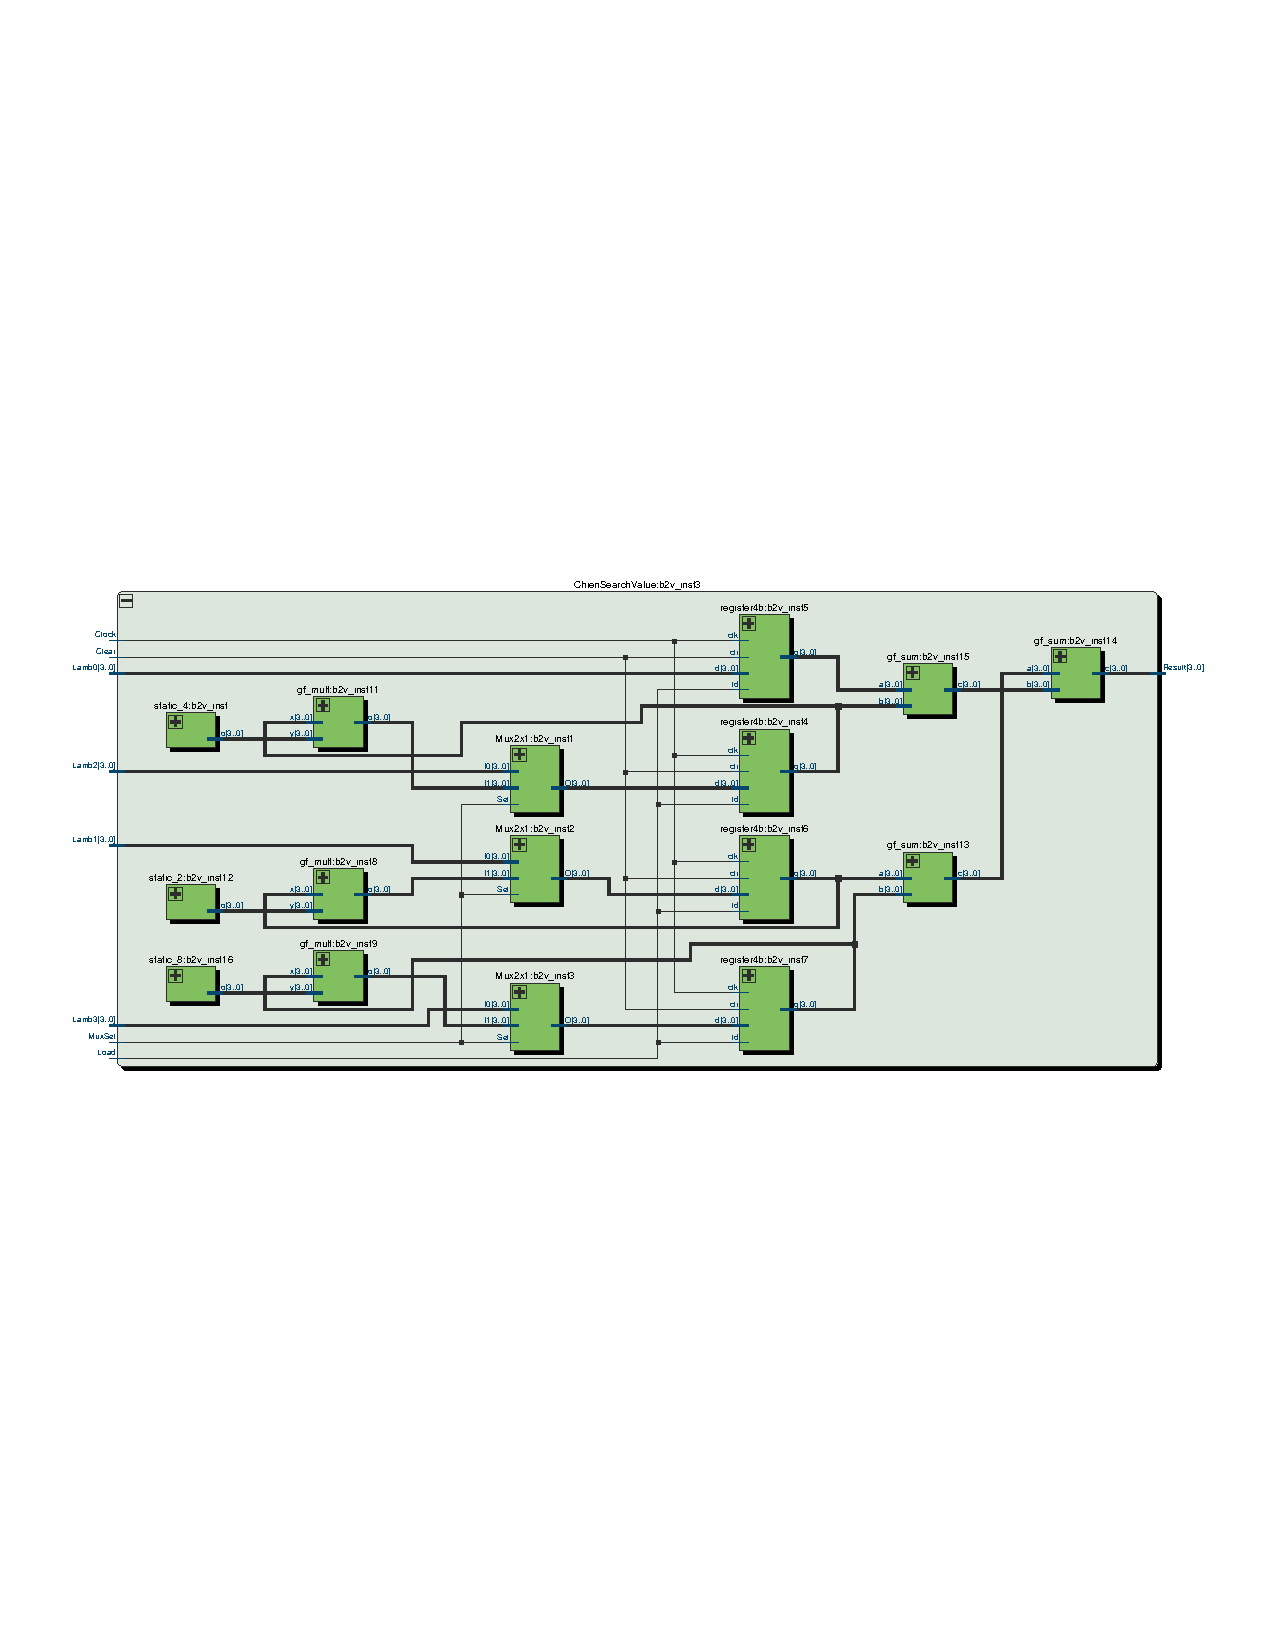
\includegraphics[width=1\textwidth]{RS/ChienValueRTL.pdf}
		\legend{}
	\end{figure}
	
	Pode-se observar que ambos funcionam com cálculo incremental. A cada ciclo, o valor de registradores é atualizado com o uso das raízes do polinômio codificador e dos coeficientes já apontados. As suas saídas vão diretamente para o módulo de Forney, uma delas indicando se deve-se corrigir o símbolo de mensagem, e outra indicando qual o valor da correção, que somado ao valor da mensagem corrigi quaisquer erros. É importante apontar que caso haja mais do que 4 símbolos com erros, nenhuma correção será feita, o que configura a condição para descarte do bloco recebido. É possível neste circuito observar esse processo com a identificação de síndromes diferentes de zero, com o sinal "errorsyndrome" na \autoref{fig_forney_sim}. Considerando que o sinal está na posição alta, significa que pelo menos um bit de alguma das síndromes é diferente de 0, e portanto a mensagem deve ser corrigida. 
	
	\begin{figure}[!htb]
		\caption{\label{fig_forney_sim} Simulação do módulo de Forney}
		\centering
		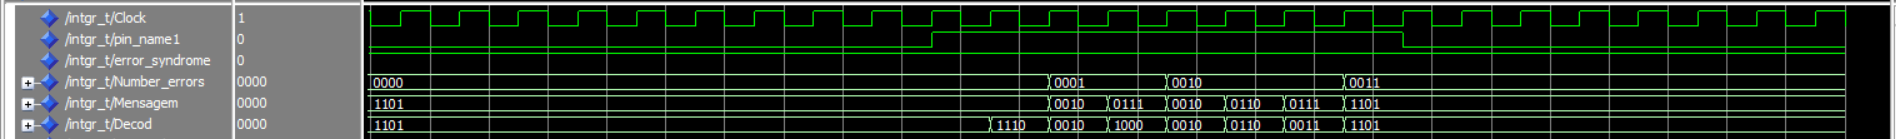
\includegraphics[width=1\textwidth]{RS/Sim_forney.PNG}
		\legend{}
	\end{figure}
	
	Por outro lado, caso haja mais de 4 símbolos com erro, nenhuma correção será feita, portanto contabiliza-se o número de correções feitas até então. Se for identificado um erro com as síndromes e não for contada nenhuma correção no módulo de Forney, temos duas condições suficientes para afirmar que o bloco deve ser descartado e este não pode ser corrigido através do método de Reed Solomon. No exemplo anterior, o número de erros corrigidos é inferior a 5, portanto a mensagem final está correta e pode sair da camada física PHY I. Caso a mensagem seja descartada, é necessário que se envie novamente pelo transmissor.
	
	% ---
	\section{Hardware}
	% ---
	A seção abaixo discorrerá sobre a aplicação dos métodos estudados nos capítulos anteriores para Hardware.
	Antes de iniciar a execução do trabalho, foram estabelecidas algumas decisões de projeto:
	
	* formato de lista *
	Única fonte de alimentação de 5V.
	Implementação de um circuito apenas para a camada PHY I da norma, fixando a frequência de operação a 200kHz.
	
	. . .
	
	
	\subsection{Transmissor}
	
	\subsubsection{Conversor Digital-Analógico}
	Com os estudos feitos no \autoref{method-hardware-conv-da}, é possível especificar os requisitos reais para o transistor de potência:

	\begin{itemize}
		\item Tensão de base/gate compatível com 3.3V;
		\item Corrente de saída compatível com LED de alta potência, no mínimo 750mA;
		\item Resposta de base/gate a $V_{on(FPGA)}$ de no máximo 1us;
	\end{itemize}
	
	Alguns dos parâmetros são decisões de projeto, como a utilização de níveis TTL para chaveamento do transistor (3.3V ou 5V), e outros são requisitos da norma IEEE, como frequência de operação a 200kHz. Especialmente no segundo caso, é importante escolher um transistor com $T_{rise}$ e $T_{fall}$ de no mínimo 10-100 vezes menor que o período da onda transmitida - no caso $5\mu$$s/100 = 50ns$. Se o transistor não chavear rápido suficiente, é possível que a onda fique alterada. Em alguns casos é possível que fique semelhante a uma onda dente de serra.
	
	O componente escolhido foi um MOSFET de Potência, mais especificamente o IRLZ14, pois é um transistor de nível lógico, pois tem o GATE compatível com voltagens de microcontrolador. 
	
	\begin{figure}[htb]
		\caption{\label{fig_transfer_carac_irlz14} Características de transferência do MOSFET de potência IRLZ14.}
		\centering		%  trim={<left> <lower> <right> <upper>} 
		
\includegraphics[page=3, width=0.5\textwidth, trim={12cm 16.5cm 2.2cm 5cm}, clip]{circuits/irlz14.pdf}
		\legend{Fonte: \cite{datasheet-irlz14}}
	\end{figure}

	De acordo com função de transferência da \autoref{fig_transfer_carac_irlz14}, a VGS=3.3V é permitida uma corrente de dreno de 2A. A datasheet também especifica parâmetros de resposta dinâmica do circuito, como seu $T_{rise}$, $T_{fall}$, que estão disponibilizados na tabela abaixo.
	
	\begin{table}[ht]
		\caption{Características Dinâmicas do MOSFET IRLZ14}
		\centering
		\begin{tabular}{c c}
			\hline
			Parâmetro  & Valor  \\ \hline
			$T_{rise}$ & 110 ns \\
			$T_{fall}$ & 26 ns  \\ \hline
		\end{tabular}
		\label{tab_irlz14_timing}
		\legend{Fonte: Vishay Siliconix.}
	\end{table}

	\subsubsection{Transmissão de Luz}
		
	Para realizar a transmissão de luz a distâncias de pelo menos um metro, será necessária a utilização de um LED de potência. Esse LED deverá atender a requisitos de altas frequência e resposta luminosa de acordo com seu chaveamento. Procuranto satisfazer tais parâmetros, o componente escolhido foi da OSRAM, o LUW W5-AM.

	Utilizando o circuito polarizador do LED da \autoref{fig_led_circuit}, é necessário calcular o valor da resistência de $R_{LIMIT}$. O LED permite no máximo 1000mA de corrente de polarização, mas não é desejável trabalhar na região limite de corrente, portanto o circuito será projetado para funcionar a 500mA. Como a voltagem de operação é de 5V, utilizando a Lei de Ohm:
	\begin{equation}
	R_{LIMIT} = 5V \cdot 500mA = 2.5\Omega
	\end{equation}
	
	\subsubsection{Versões Anteriores}
	
	Devido a falta de conhecimento do comportamento de transistores e da resposta de todos os componentes a frequência de 200kHz, foram projetados vários circuitos que não satisfaziam o formato de onda desejado. Abaixo são exemplificadas algumas versões implementadas, juntamente com os motivos de terem sido abandonadas.
	
	\paragraph{Filtro da Ponta de Prova}
	\begin{figure}[htb]
		\caption{\label{fig_transmitter_lify_circuit_fail0} Circuito de transmissão com filtro de ponta de prova. }
		\centering		%  trim={<left> <lower> <right> <upper>} 
		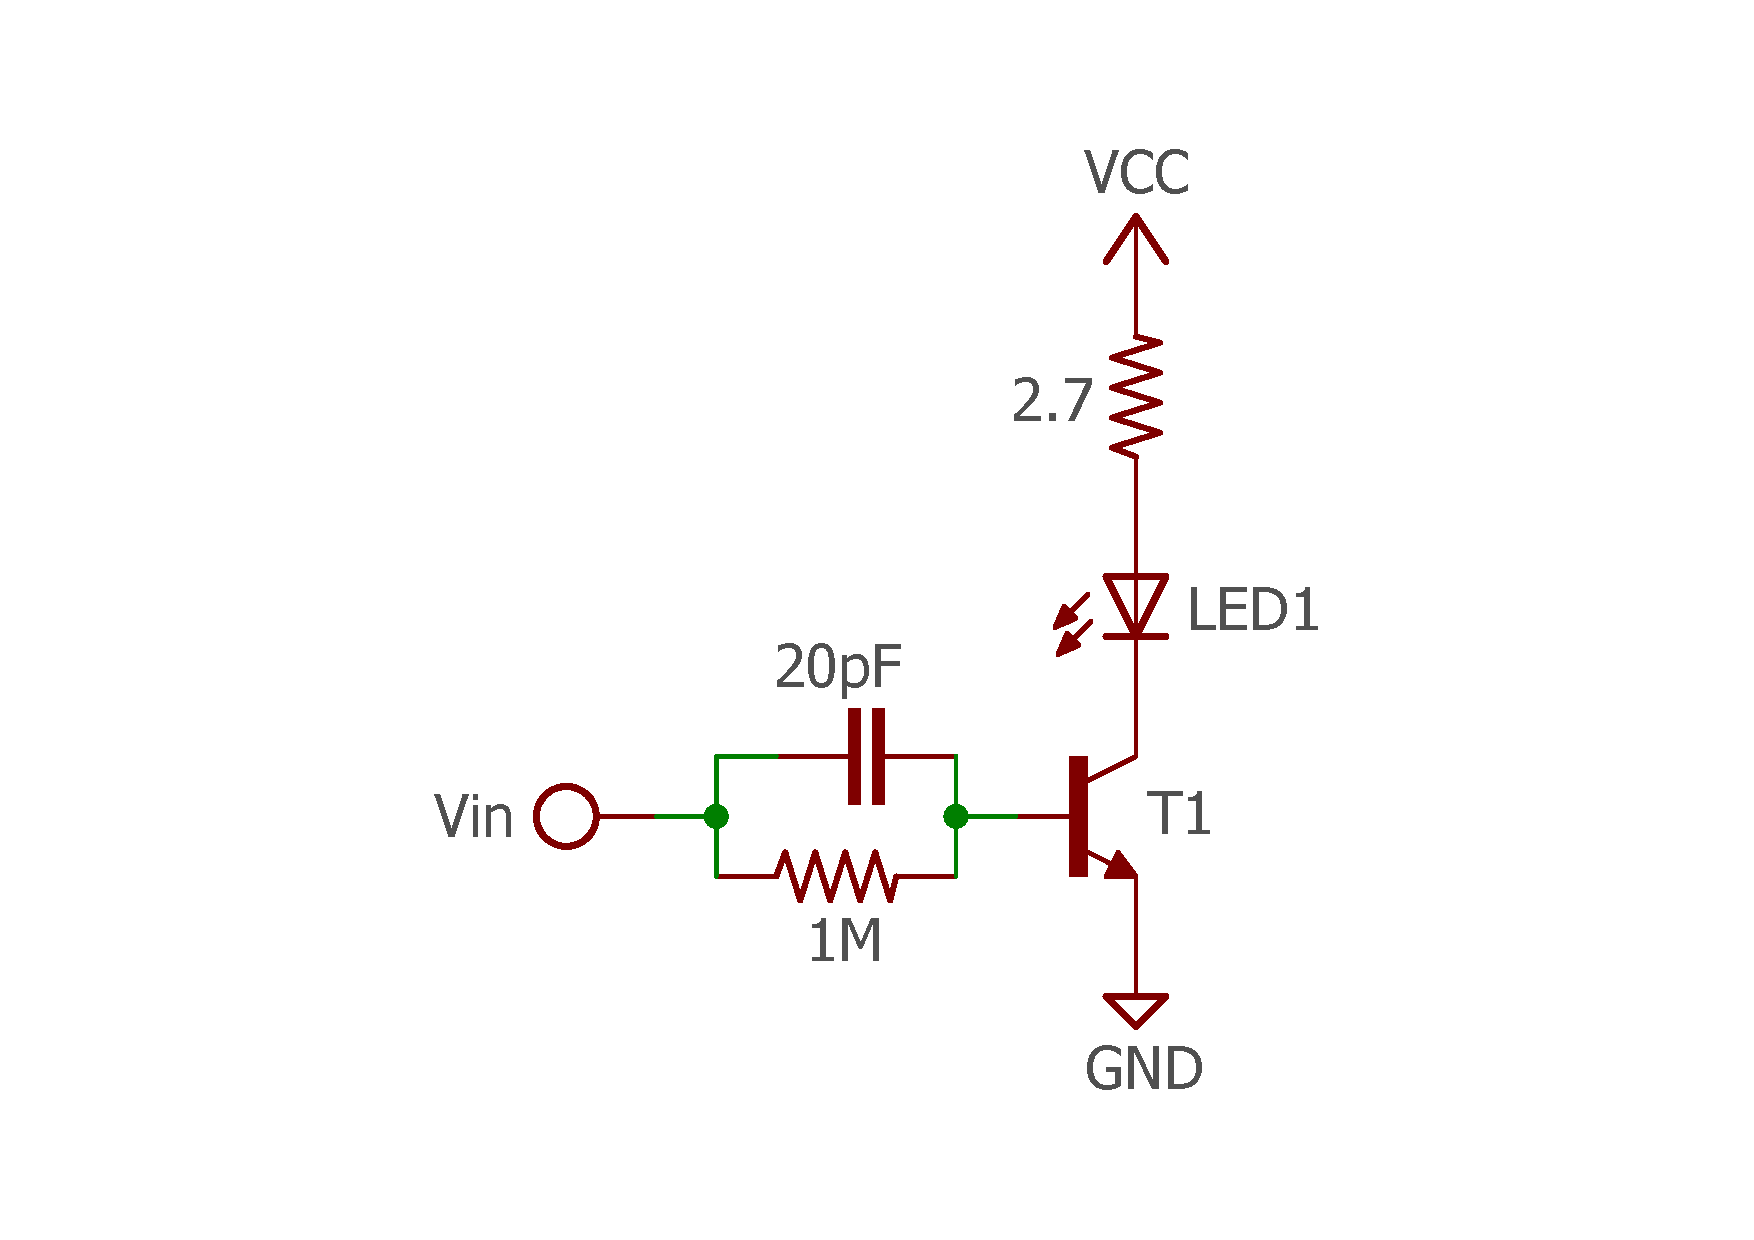
\includegraphics[width=0.7\textwidth, trim={2cm 1cm 2cm 2cm}, clip]{circuits/transmitter_fail0.pdf}
		\legend{Fonte: Autores}
	\end{figure}
	O primeiro problema que o projeto do transmissor encontrou foi o comportamento de subamortecimento nos terminais do LED. Ele utiliza um circuito semelhante ao utilizado em pontas de provas para filtrar ruídos e é conectado em série com a entrada do transmissor, como visto na \autoref{fig_transmitter_lify_circuit_fail0}.
	\begin{figure}[htb]
		\caption{\label{fig_transmitter_lify_circuit_fail0_rl} Comportamento do circuito de transmissão com filtro de ponta de prova em série com a entrada. A onda azul é saída do gerador de funções enquanto a onda amarela é a tensão submetida ao LED. Observa-se o comportamento de subamortecimento em ambas.}
		\centering		%  trim={<left> <lower> <right> <upper>} 
		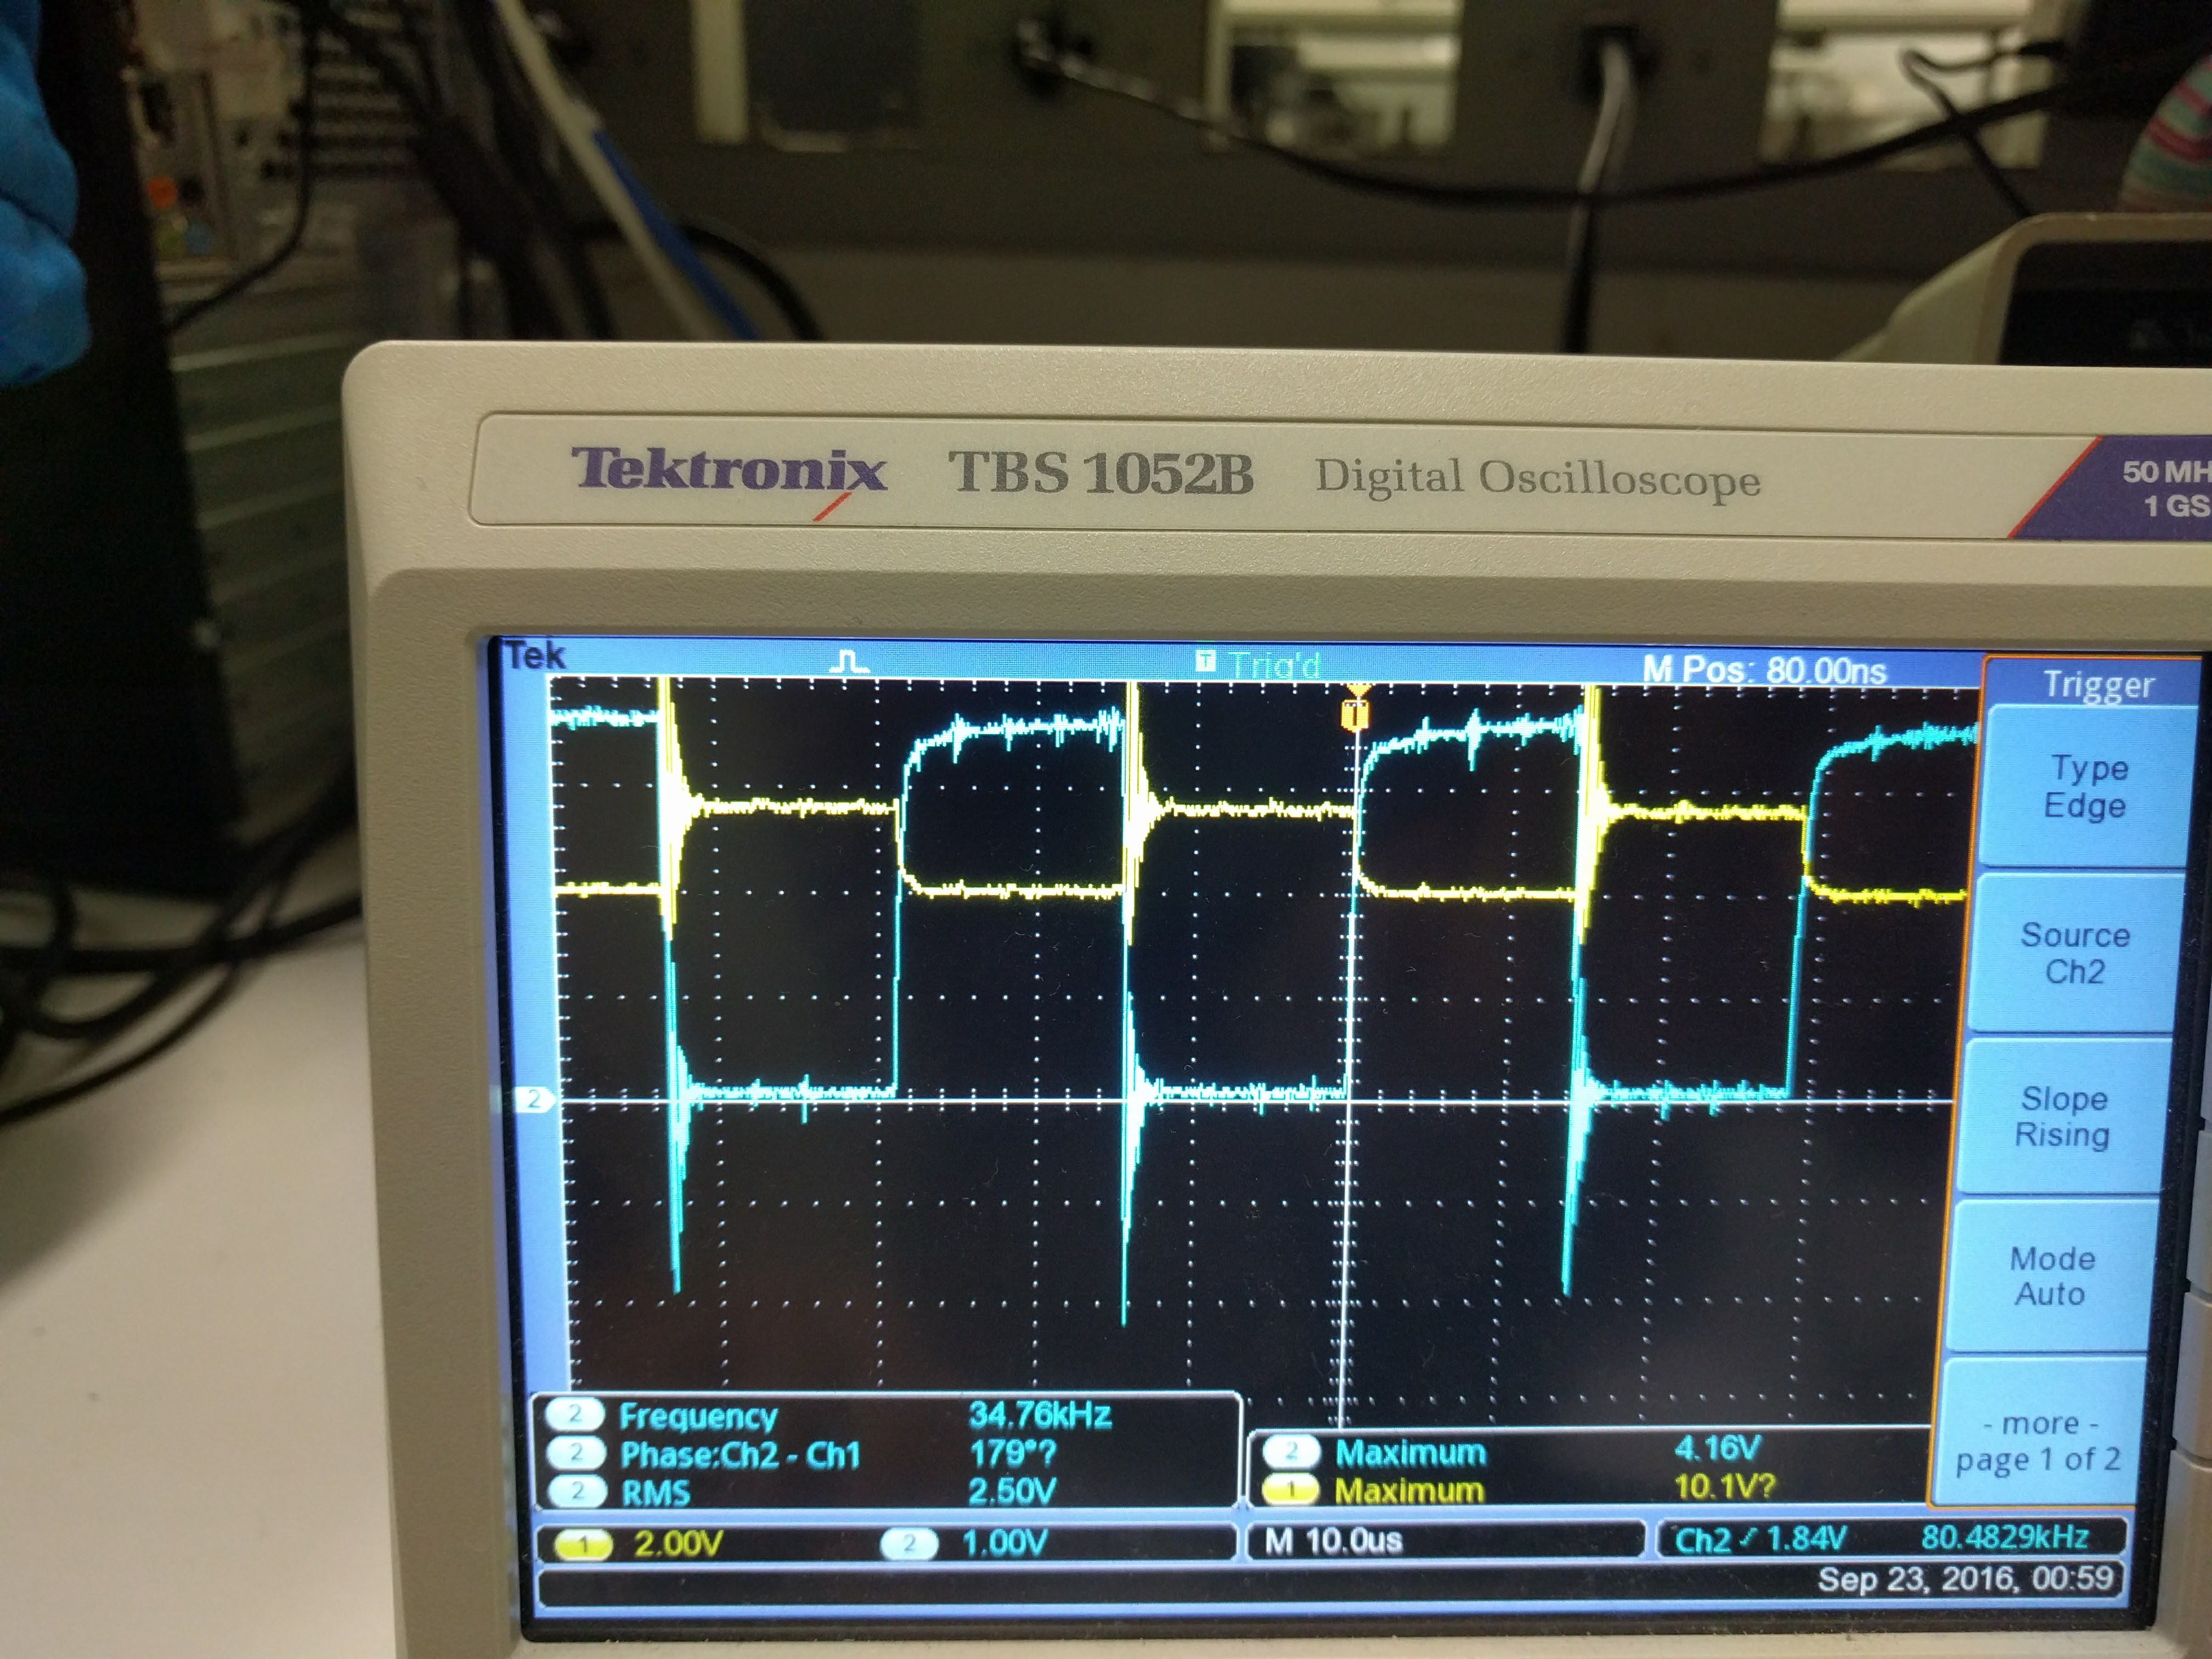
\includegraphics[width=0.5\textwidth, trim={30cm 0cm 2cm 40cm}, clip]{circuits/photos/TX_probe_result.jpg}
		\legend{Fonte: Autores}
	\end{figure}

	A saída dessa implementação é mostrada na \autoref{fig_transmitter_lify_circuit_fail0_rl} e não foi satisfatória. O primeiro ponto a se notar é que a frequência de operação era baixa, no caso 80kHz - ainda 120kHz abaixo da especificação da velocidade da camada PHY I. Além dessa frequência a forma de onda se distorcia demais. O segundo ponto observado foi o fato de que houve uma resposta de subamortecimento tanto na entrada quanto na saída. Atribuiu-se esses efeitos a capacitâncias parasitas no LED e no transistor de potência.
	
	O transistor de potência possui capacitância devido a separação de suas placas. Seu valor é significativo e é até especificado na datasheet. Para o IRLZ14, a capacitância de entrada é 400pF e de saída 170pF. Esses valores devem ser levados em conta ao polarizar tal componente. 

	No caso do LED, esse comportamento é mais complexo. A frequências altas, seu chaveamento cria um capacitor entre seus terminais, devido a sua arquitetura semicondutora. É possível observar esse comportamento capacitivo tanto em um LED de baixa potência quando de alta. Na prática, a tensão sob o LED não diminui acompanhando a tensão submetida a ele, e isso causa o comportamento indesejável visto, como os picos na onda amarela.
	
	A forma de onda gerada por esse circuito é muito boa, porém os picos de voltagem de até o dobro de $2 \cdot V_{CC} = 10V$ com certeza danificam os componentes. Essa versão foi descartada por esse motivo (como pode-se observar em no osciloscópio - \textbf{Maximum 10.1V}). 
	
	Em um teste unitário, foi observado o comportamento do chaveamento de um resistor $R_{L}$ a 200kHz, removendo completamente o LED do sistema. A saída observada era exatamente igual a entrada. Colocando um LED em série com o resistor adicionava o comportamento subamortecido, portanto conclui-se que a anomalia é atribuida ao LED.
	
	\paragraph{Aumento da Frequência}

	O aumento da frequência de operação a $f_{OP} = 200kHz$ causa um subamortecimento substancialmente maior. Observa-se na \autoref{fig_transmitter_lify_circuit_fail1_r1}, que provém de circuito sem o filtro da ponta de prova na \autoref{fig_transmitter_lify_circuit_fail1}.
	\begin{figure}[htb]
		\caption{\label{fig_transmitter_lify_circuit_fail1} Circuito de transmissão sem o filtro de ponta de prova.}
		\centering		%  trim={<left> <lower> <right> <upper>} 
		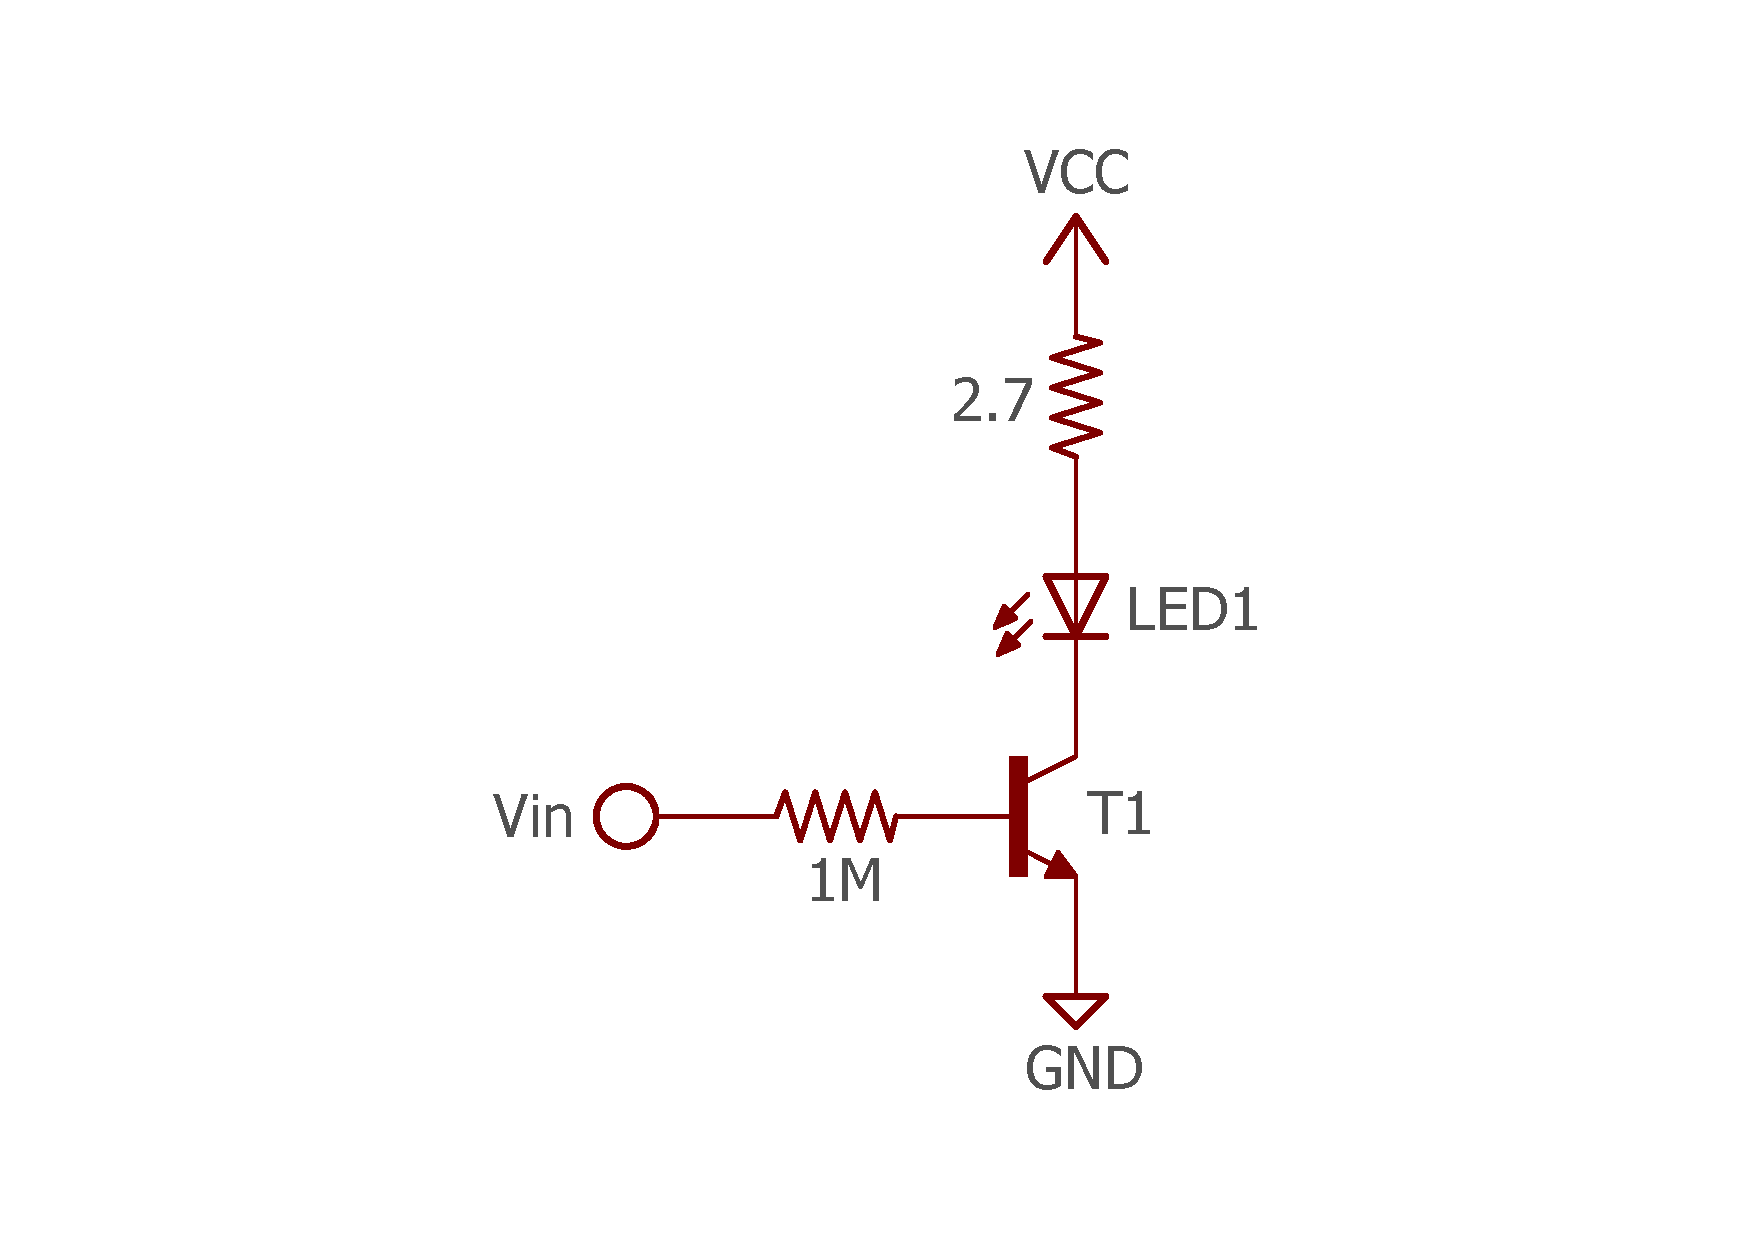
\includegraphics[width=0.5\textwidth, trim={2cm 1.5cm 2cm 2cm}, clip]{circuits/transmitter_fail1.pdf}
		\legend{Fonte: Autores}
	\end{figure}
	
	\begin{figure}[htb]
		\caption{\label{fig_transmitter_lify_circuit_fail1_r1} Operação de circuito transmissor sem ponta de prova. A onda amarela representa voltagem no LED sem filtro de ponta de prova em frequências mais altas. O gerador de funções é medido e gera a forma de onda verde.}
		\centering		%  trim={<left> <lower> <right> <upper>} 
		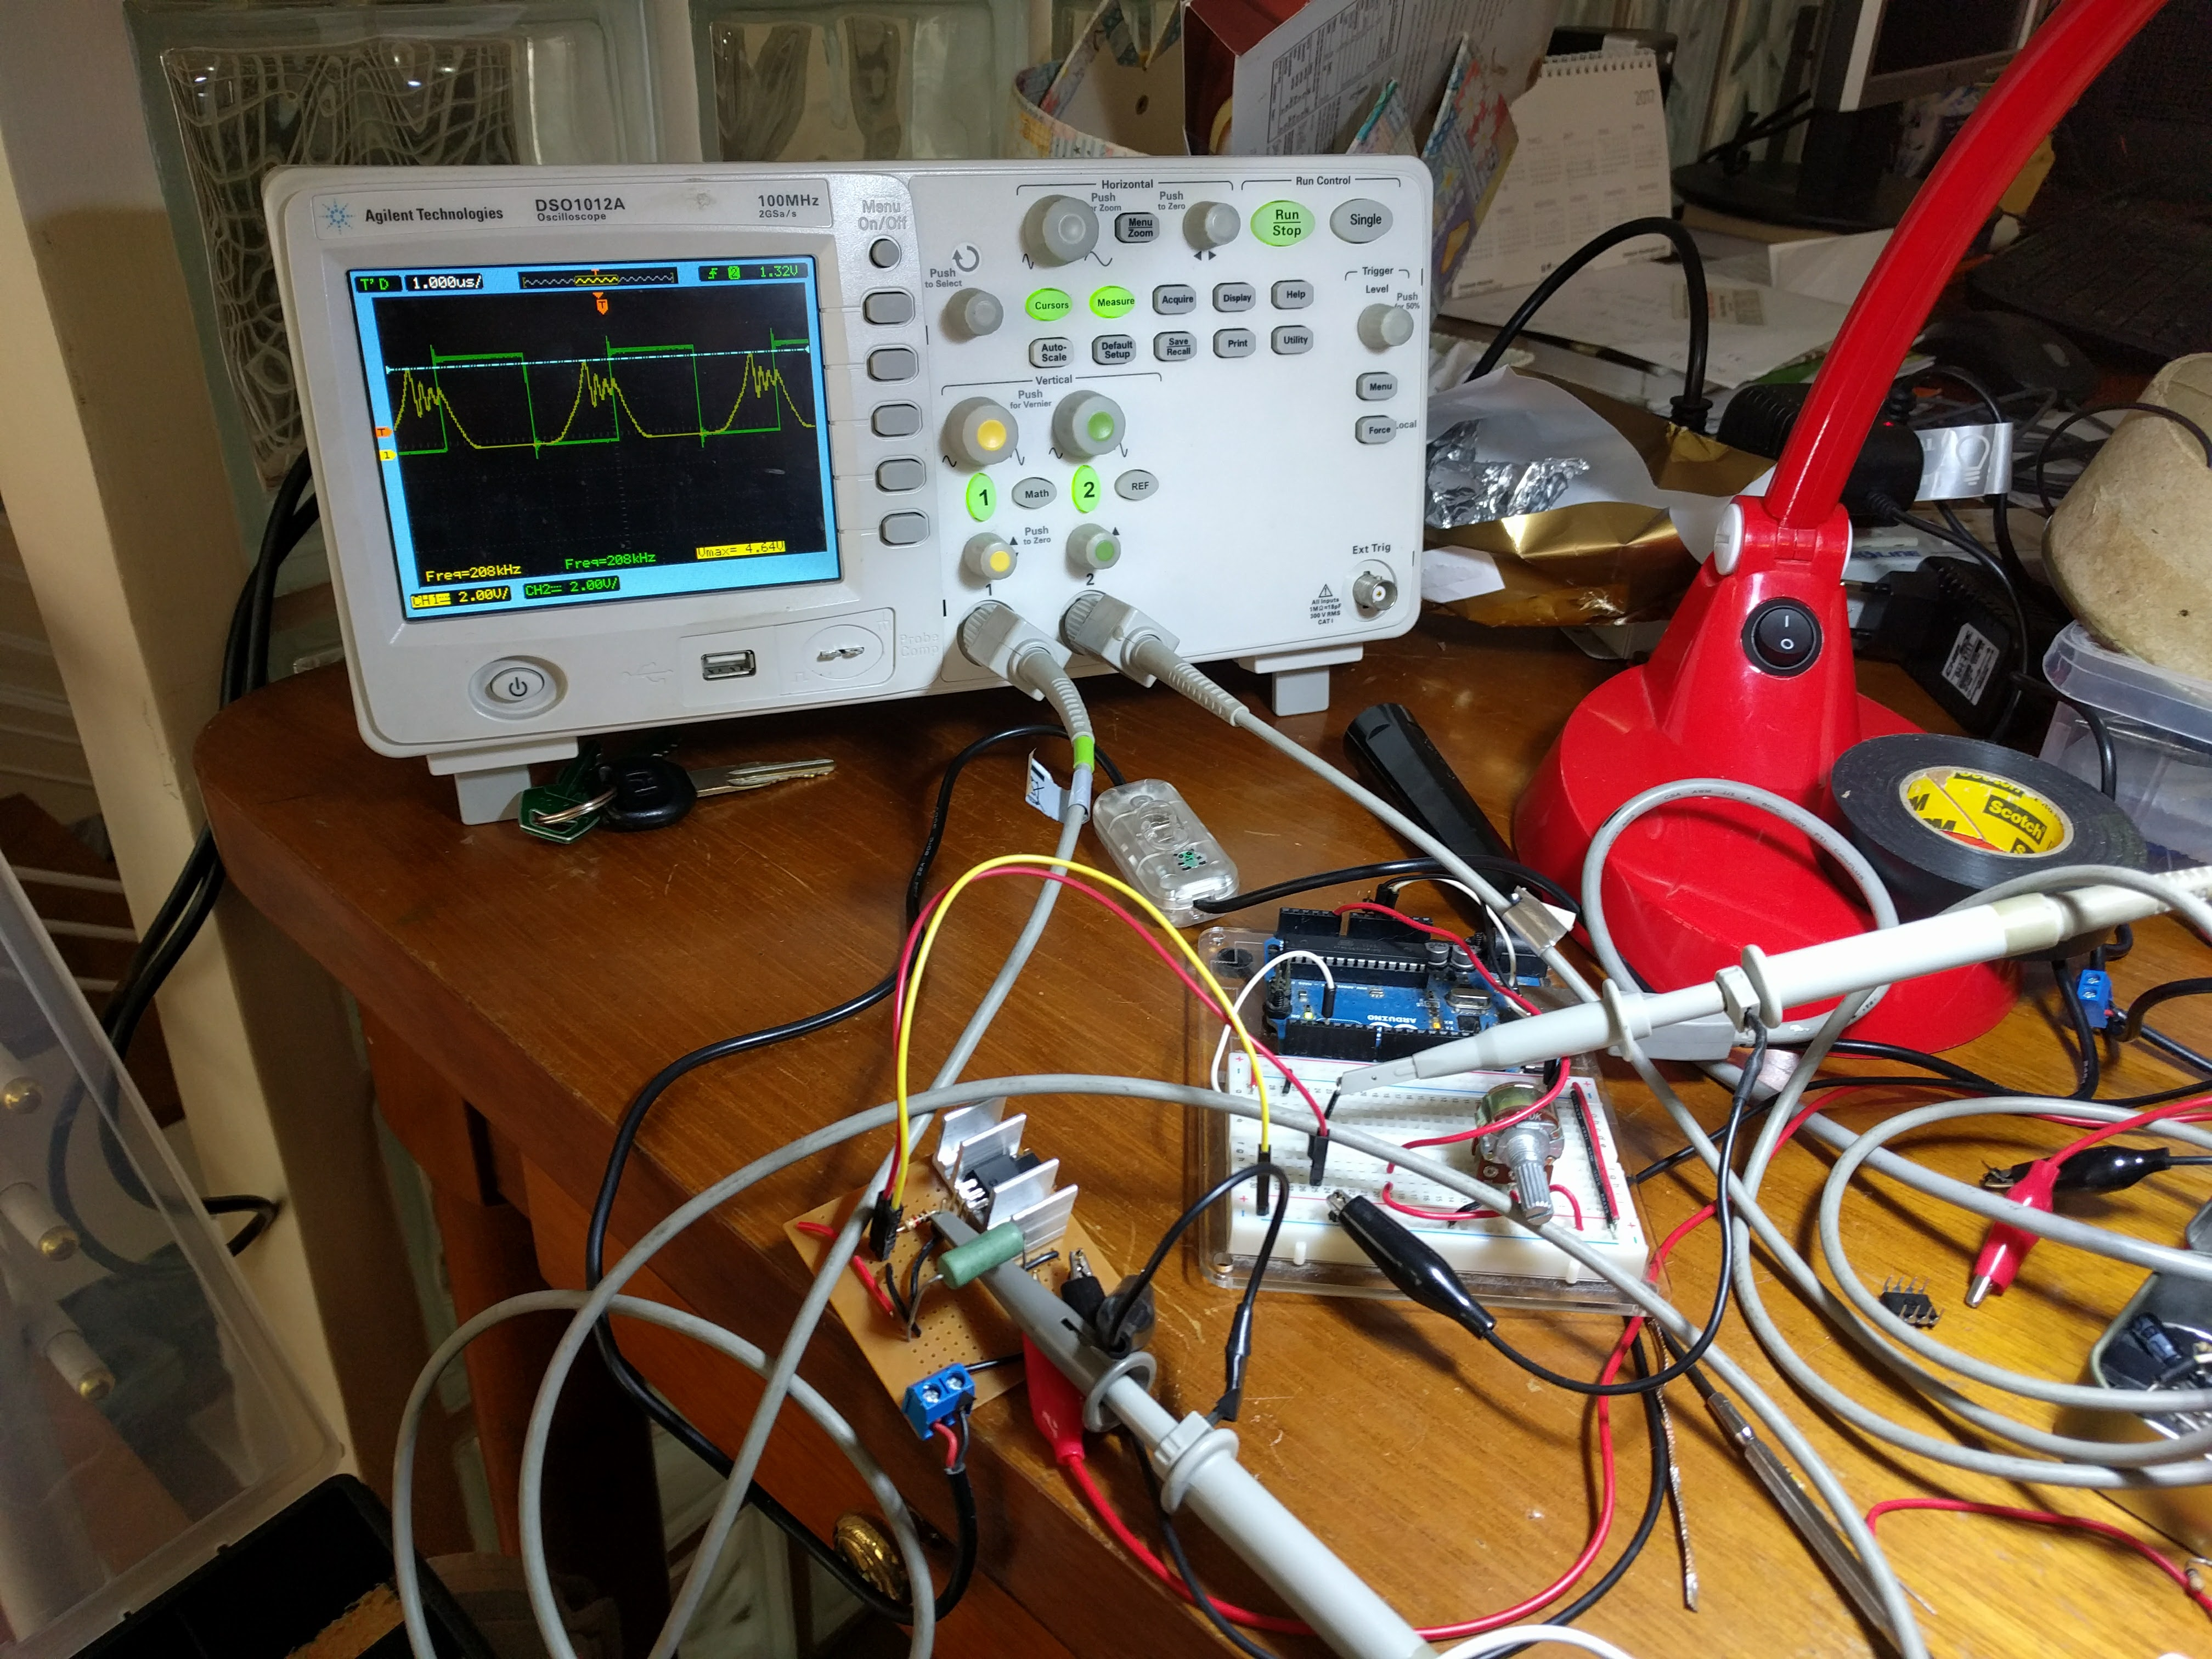
\includegraphics[width=0.5\textwidth, trim={20cm 65cm 85cm 10cm}, clip]{circuits/photos/TX_200k_without_filter.jpg}
		\legend{Fonte: Autores}
	\end{figure}
	Nesse caso é muito mais evidente o amortecimento visto na onda. Atribui-se esse comportamento a componente capacitiva ao chavear o LED. No entanto, observa-se que não há feedback do circuito na saída do gerador de funções, fato observado na última versão do circuito. O capacitor colocado adicionava um nível de complexidade desnecessário ao circuito, pois se carregava com oscilação da entrada. 
	
	Além disso, ele não preserva a forma de onda da entrada. Ainda é possível refinar mais a solução.
	
	\paragraph{Final - Filtro Passa-Altas}
			
	\begin{figure}[htb]
		\caption{\label{fig_transmitter_lify_circuit_final} Circuito final de transmissão de dados LiCy, utilizando um filtro passa-altas.}
		\centering		%  trim={<left> <lower> <right> <upper>} 
		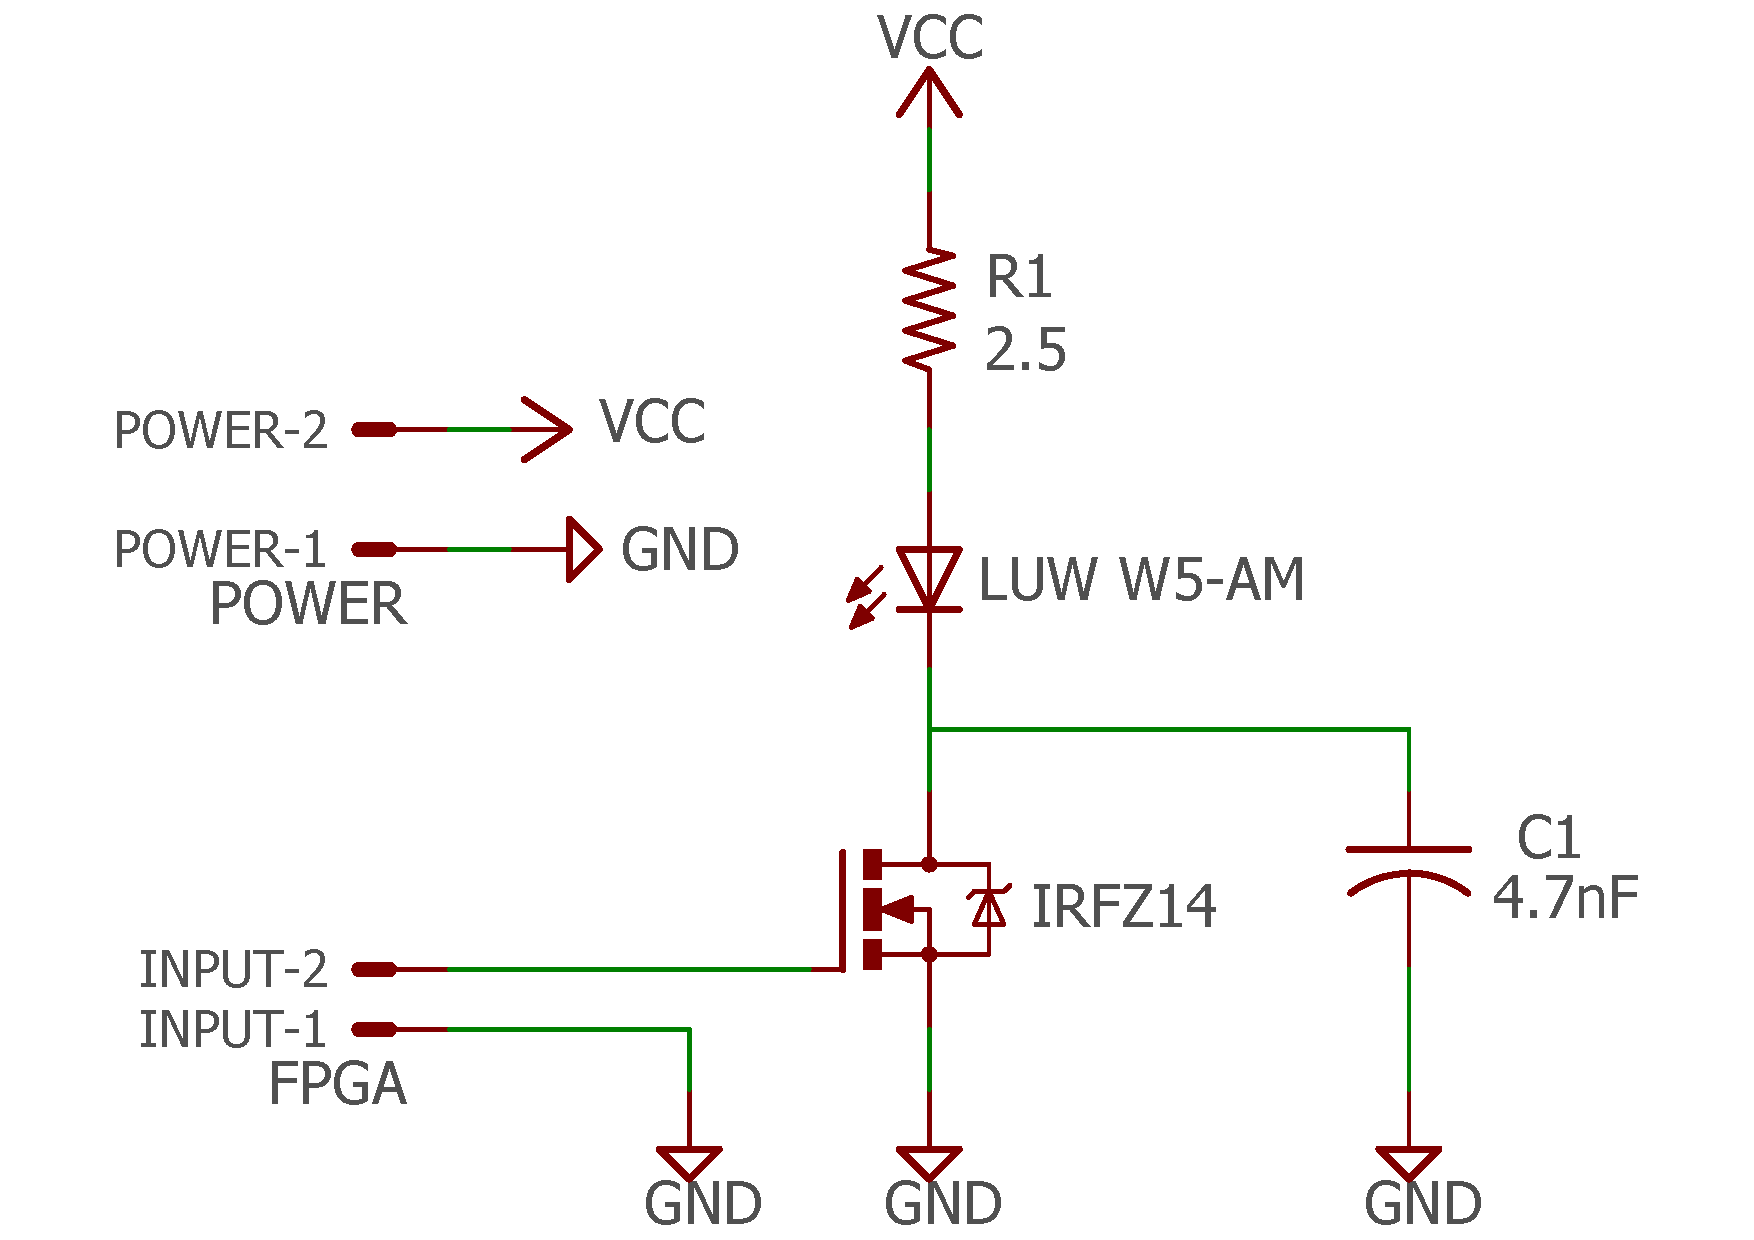
\includegraphics[width=0.7\textwidth, trim={2cm 0cm 2cm 0cm}, clip]{circuits/transmitter_lify.pdf}
		\legend{Fonte: Autores}
	\end{figure}
	
	\begin{figure}[htb]
		\caption{\label{fig_transmitter_lify_circuit_final_r1} Forma de onda após adicionar um capacitor que age como filtro passa-altas. Está defasada em 180$\degree$. }
		\centering		%  trim={<left> <lower> <right> <upper>} 
		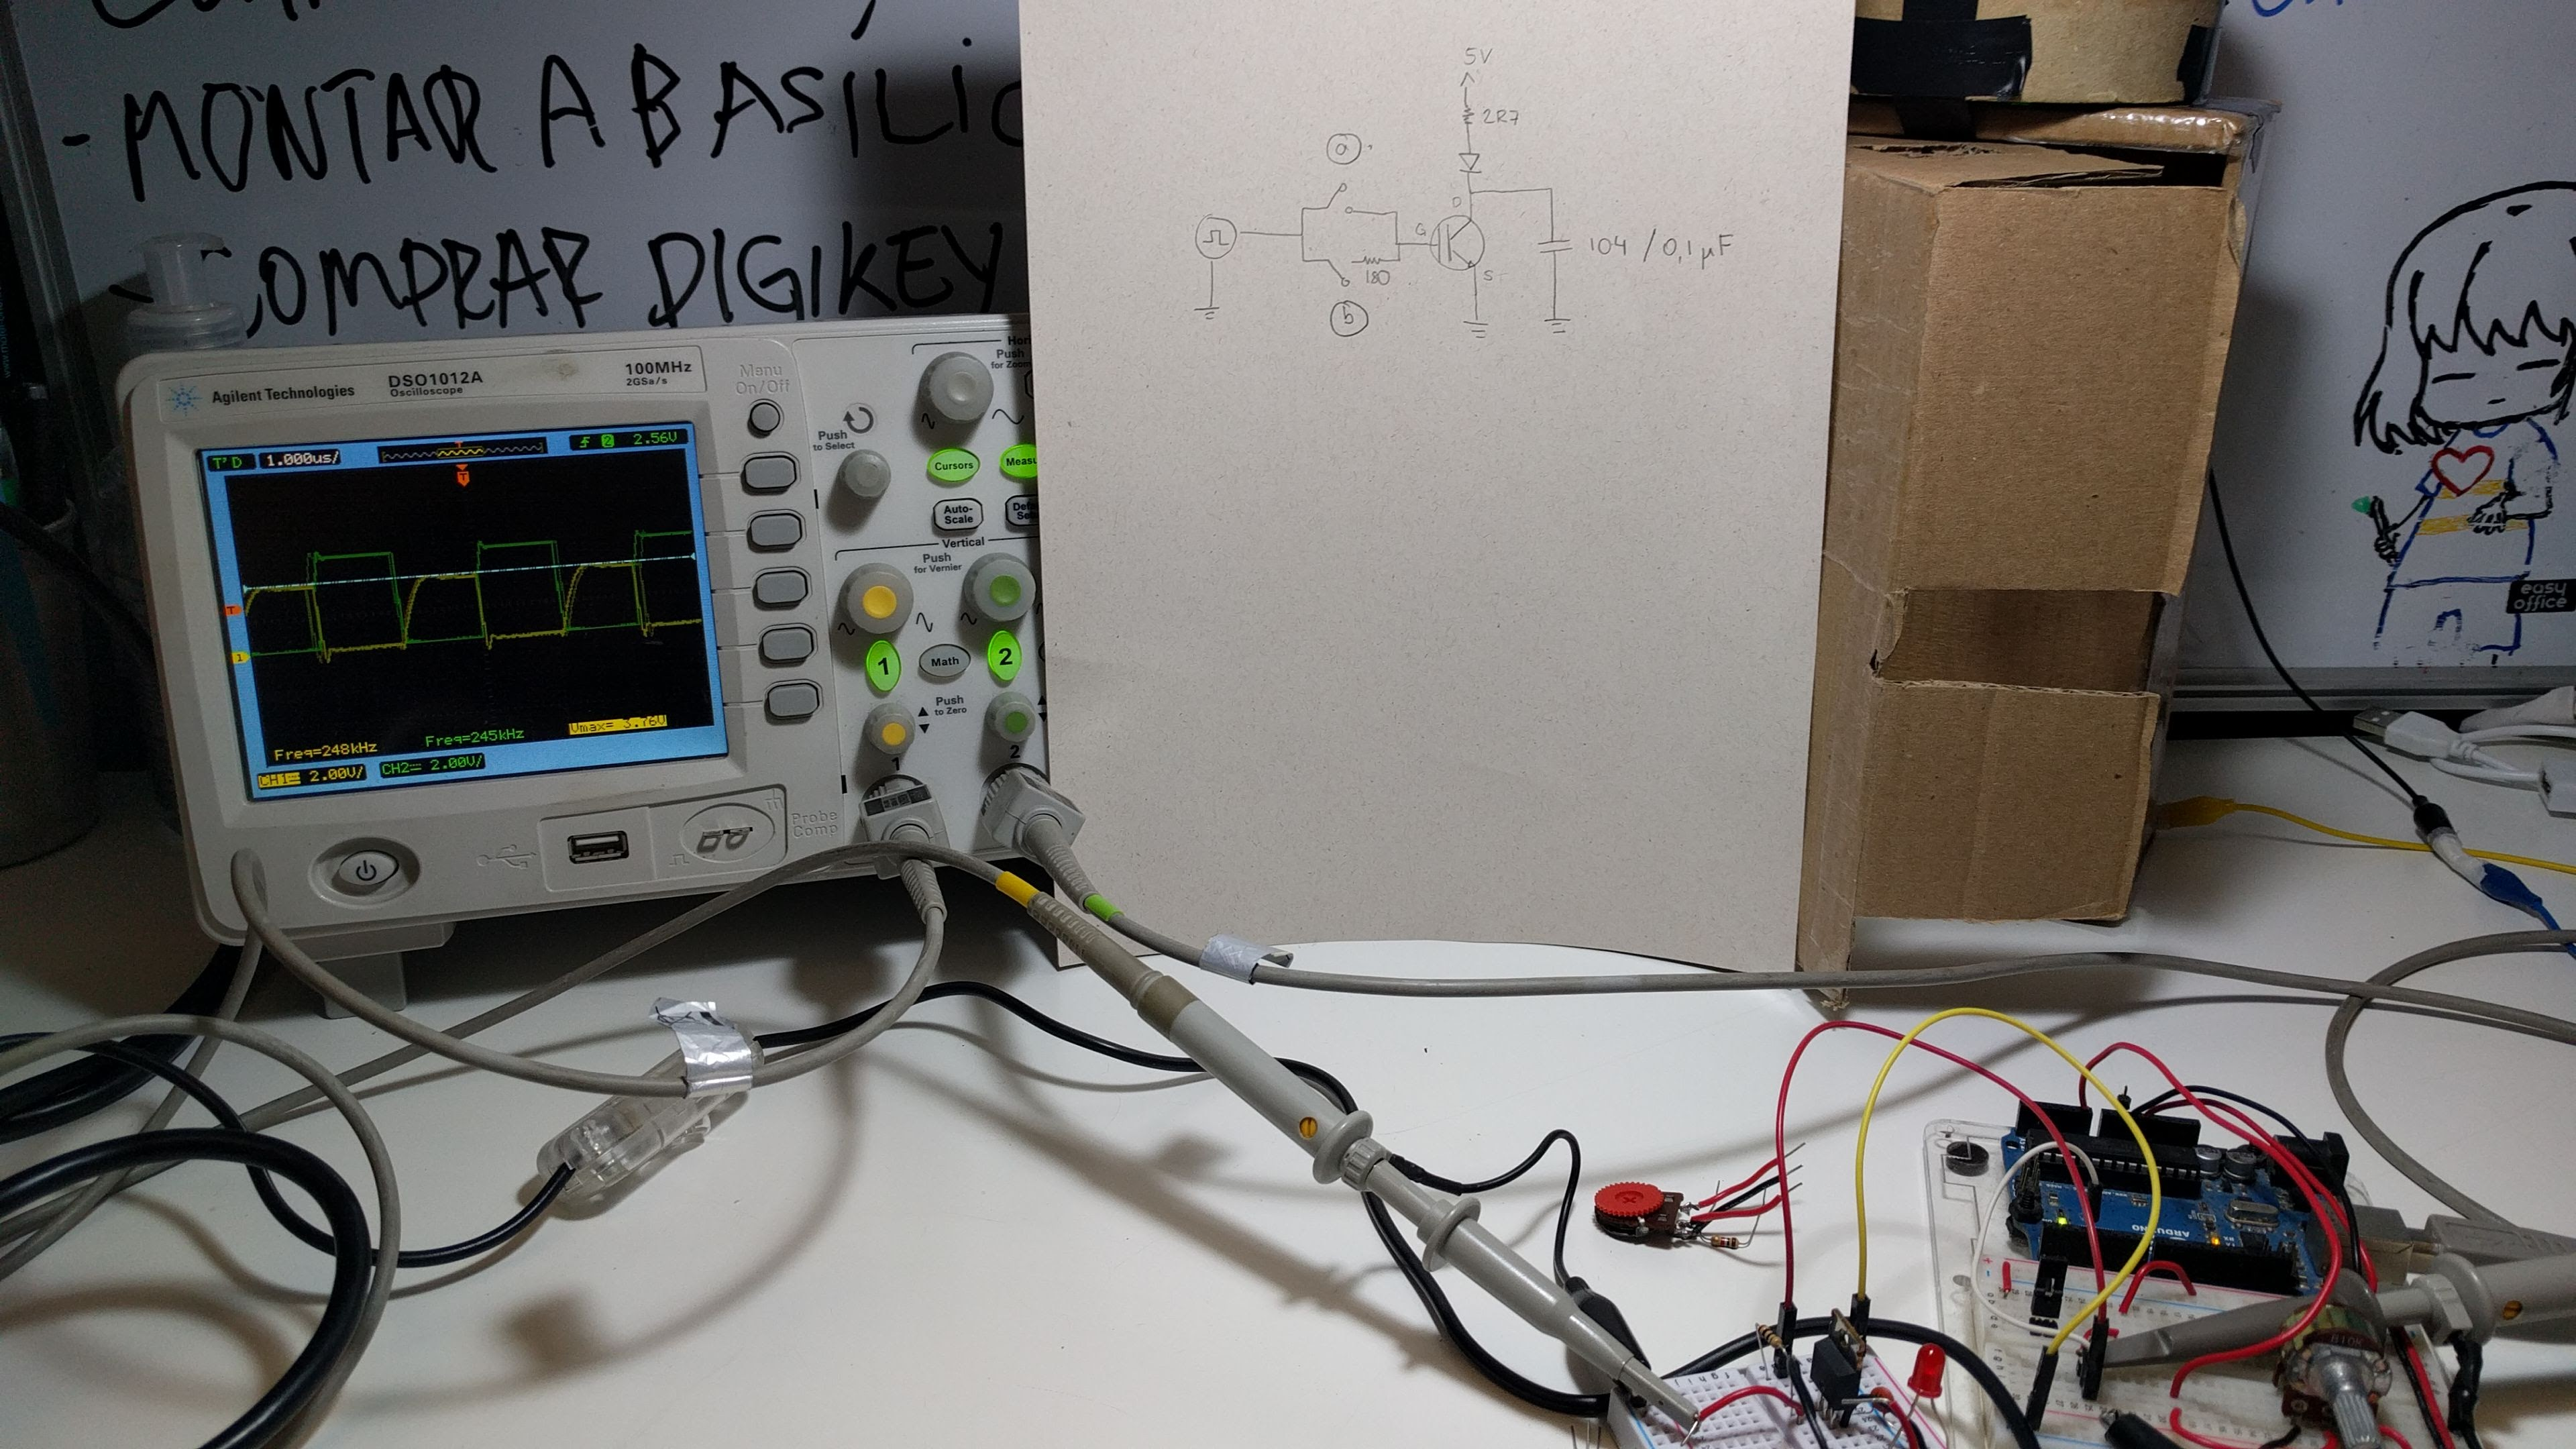
\includegraphics[width=0.5\textwidth, trim={5cm 30cm 90cm 20cm}, clip]{circuits/photos/TX_200k_with_filter.jpeg}
		\legend{Fonte: Autores}
	\end{figure}

	Por fim, realiza-se a correção dessa componente subamortecida utilizando um capacitor entre os terminais da Source do MOSFET e GND (observado em \autoref{fig_transmitter_lify_circuit_final}). Esse capacitor atua como filtro passa-altas e remove a componente AC da saída para o LED. O comportamento não fica exatamente igual à entrada, mas fica satisfatório pois o período é muito similar, chaveando o LED corretamente. A forma de onda resultante pode ser observada em \autoref{fig_transmitter_lify_circuit_final_r1}. Está defasada em 180$\degree$.

	\subsection{Receptor}
	
	A recepção será feita utilizando os conceitos apresentados nas seções \ref{method-hard-photodiode}, \ref{method-hardware-conv-ad}, \ref{method-hardware-highpass-filter}, \ref{method-hardware-dc-bias};
	
	\subsubsection{Recepção Luminosa}
	Para o recebimento luminoso, foi utilizado um circuito da \textbf{APPLICATION NOTES} da \cite{datasheet-opa380}, simplificado e esquematizado na \autoref{fig_transimpedance_amp_complex_outer}, diferente do utilizado na Metodologia (\autoref{fig_transimpedance_amp_simple}). Com $V_{bias} = 2.5V$ polarizando reversamente o fotodiodo, uma resposta mais confiável era recebida pelo componente. O valor de R1 e R2 foram  escolhidos como 1M$\Omega$ e 100k$\Omega$.
	
	\begin{figure}[htb]
		\caption{\label{fig_transimpedance_amp_complex_outer} Circuito e saída de um amplificador de impedâncias. No circuito, o fotodiodo é reversamente polarizado por $V_{bias}$. No osciloscópio, a saída está marcada em amarelo enquanto a saída do LED está em verde.}
		\begin{subfigure}{.5\textwidth}
			\centering
			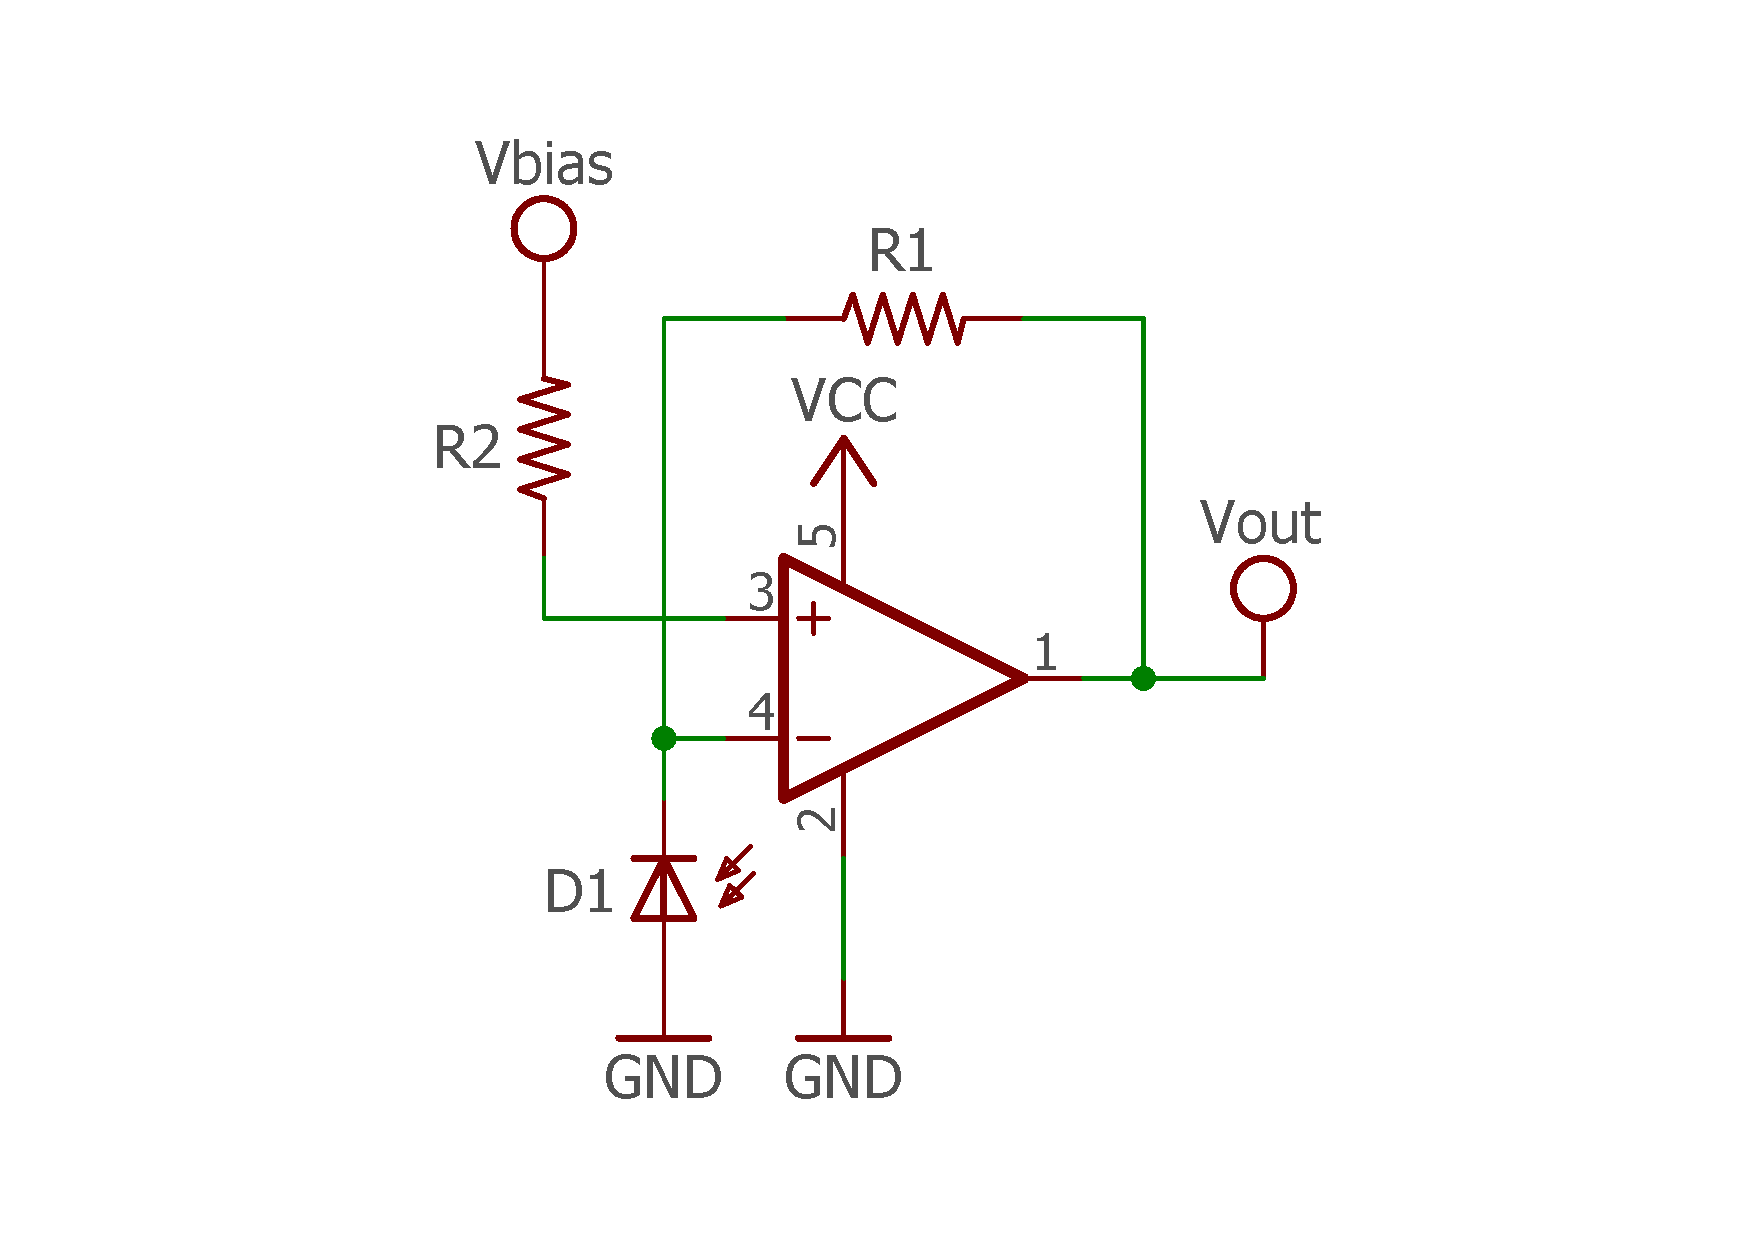
\includegraphics[width=1\textwidth, trim={1cm 1cm 1cm 2cm}, clip]{circuits/transimpedance_amp.pdf}
		\end{subfigure}
		\begin{subfigure}{.5\textwidth}
			\centering
			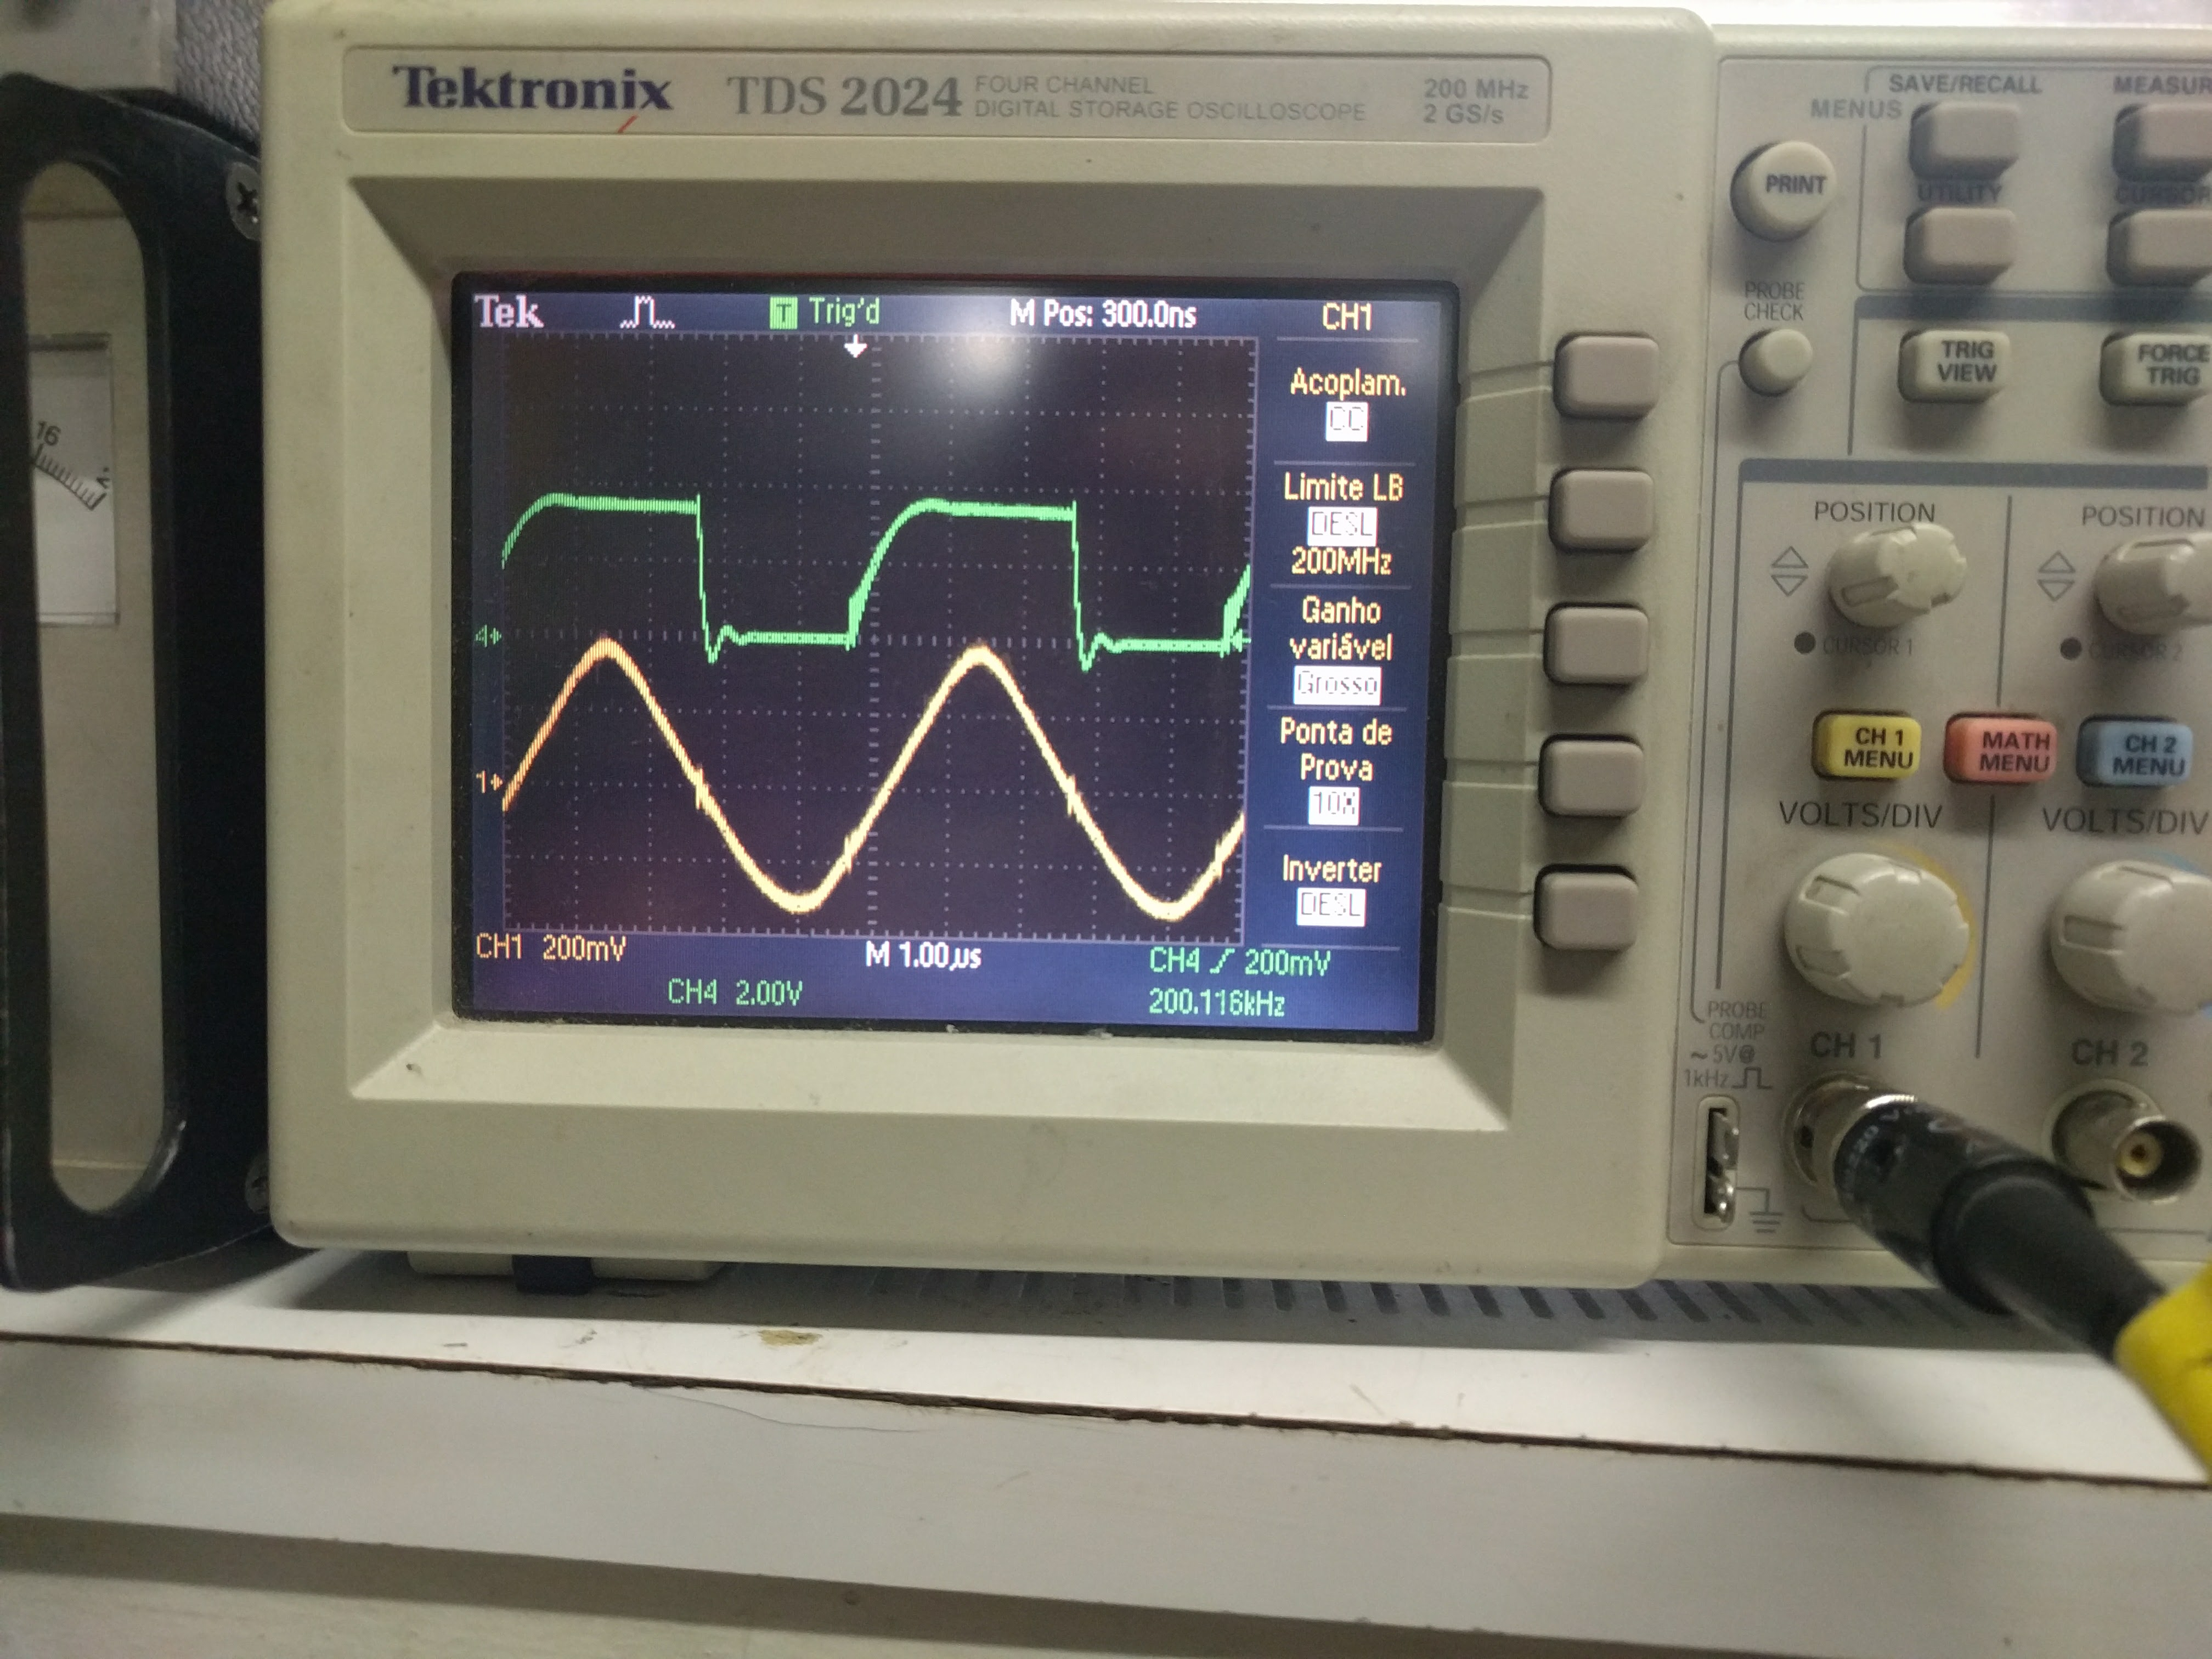
\includegraphics[width=1\textwidth, trim={25cm 35cm 40cm 15cm}, clip]{circuits/photos/RX_TIA_result.jpg}
		\end{subfigure}
		\legend{Fonte: Autores}
	\end{figure}

	No osciloscópio, a componente DC da saída do amplificador de transimpedância é zero. No entanto, esse valor é apenas zero quando o padrão da oscilação luminosa se estabiliza. Entrando em detalhes: nesse e em todos casos de teste, o receptor está sendo submetido a uma onda quadrada de $f = 200kHz$. Como a norma define Manchester como código de RLL, é providenciado balanço DC ao receptor (são transmitidos a mesma quantidade de zeros e uns). Então o fotodiodo se desestabilizará quando há movimentação dos módulos ou quando há mudança na iluminação do ambiente.
	
	Para remover esses fatores de incerteza, o circuito de passas baixas com acomplamento DC $V_{ref} = 1V$ foi projetado a partir da \autoref{plot-post-bias1v}. Para obter uma voltagem de referência de 1V foi utilizado um divisor resistivo de 12k e 47k. 
	
	\begin{equation}
	V_{out} = V_{in} \cdot \frac{12k}{12k + 47k} = V_{in} \cdot \frac{12k}{59k} \approx \frac{V_{in}}{5} = \frac{V_{CC}}{5} \approx 1V
	\end{equation}
	
	\subsubsection{Conversor Analógico-Digital}
	
	Com a onda em $V_{DC} = 1V$, é possível utilizar o comparador definido na \autoref{fig_double_comparator} para converter a onda senoidal em uma onda quadrada, com níveis compatíveis com a FPGA.
	
	A voltagem de referência do comparador deve ser a mesma que a voltagem $V_{ref}$ do filtro passa-baixas, provenientes do divisor resistivo. O circuito final integrado do receptor pode é analisado na \autoref{fig_receiver_lify_circuit_final}.

	\begin{figure}[htb]
		\caption{\label{fig_receiver_lify_circuit_final} Circuito esquemático final de recepção de dados LiCy.}
		\centering
		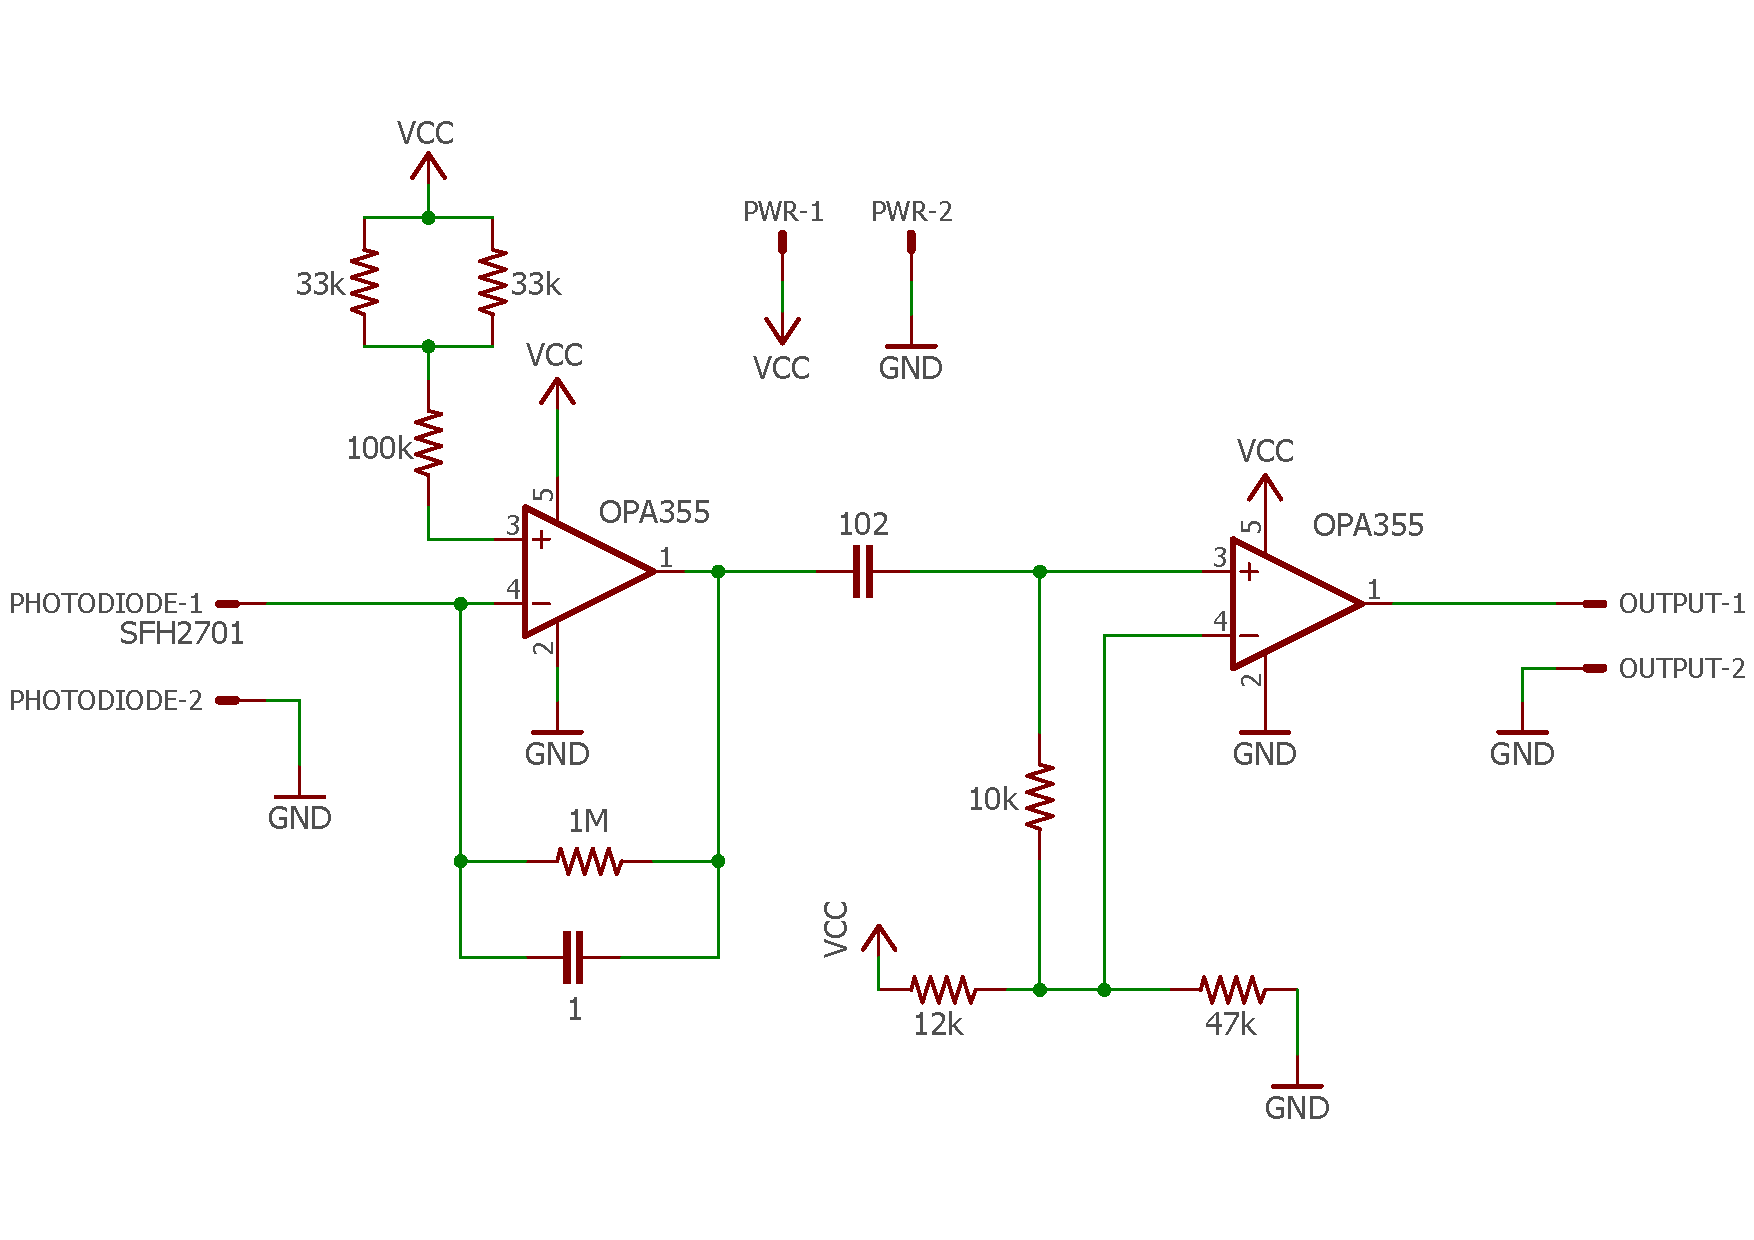
\includegraphics[width=0.7\textwidth, trim={0cm 1cm 0cm 1cm}, clip]{circuits/receiver_lify_final.pdf}
		\legend{Fonte: Autores}
	\end{figure}
	
	Os testes realizados foram bem sucedidos e resultaram na onda da \autoref{fig_receiver_lify_circuit_final_r1}. Nela é possível observar a medição do período da onda resultante convertida, que foi 4.88us, muito próximo de 5us, período para 200kHz.
	
	\begin{figure}[htb]
		\caption{\label{fig_receiver_lify_circuit_final_r1} Saída do transmissor em verde e saída digital convertida do receptor em amarelo. É possível observar uma defasagem de 90$\degree$ em relação às ondas.}
		\centering
		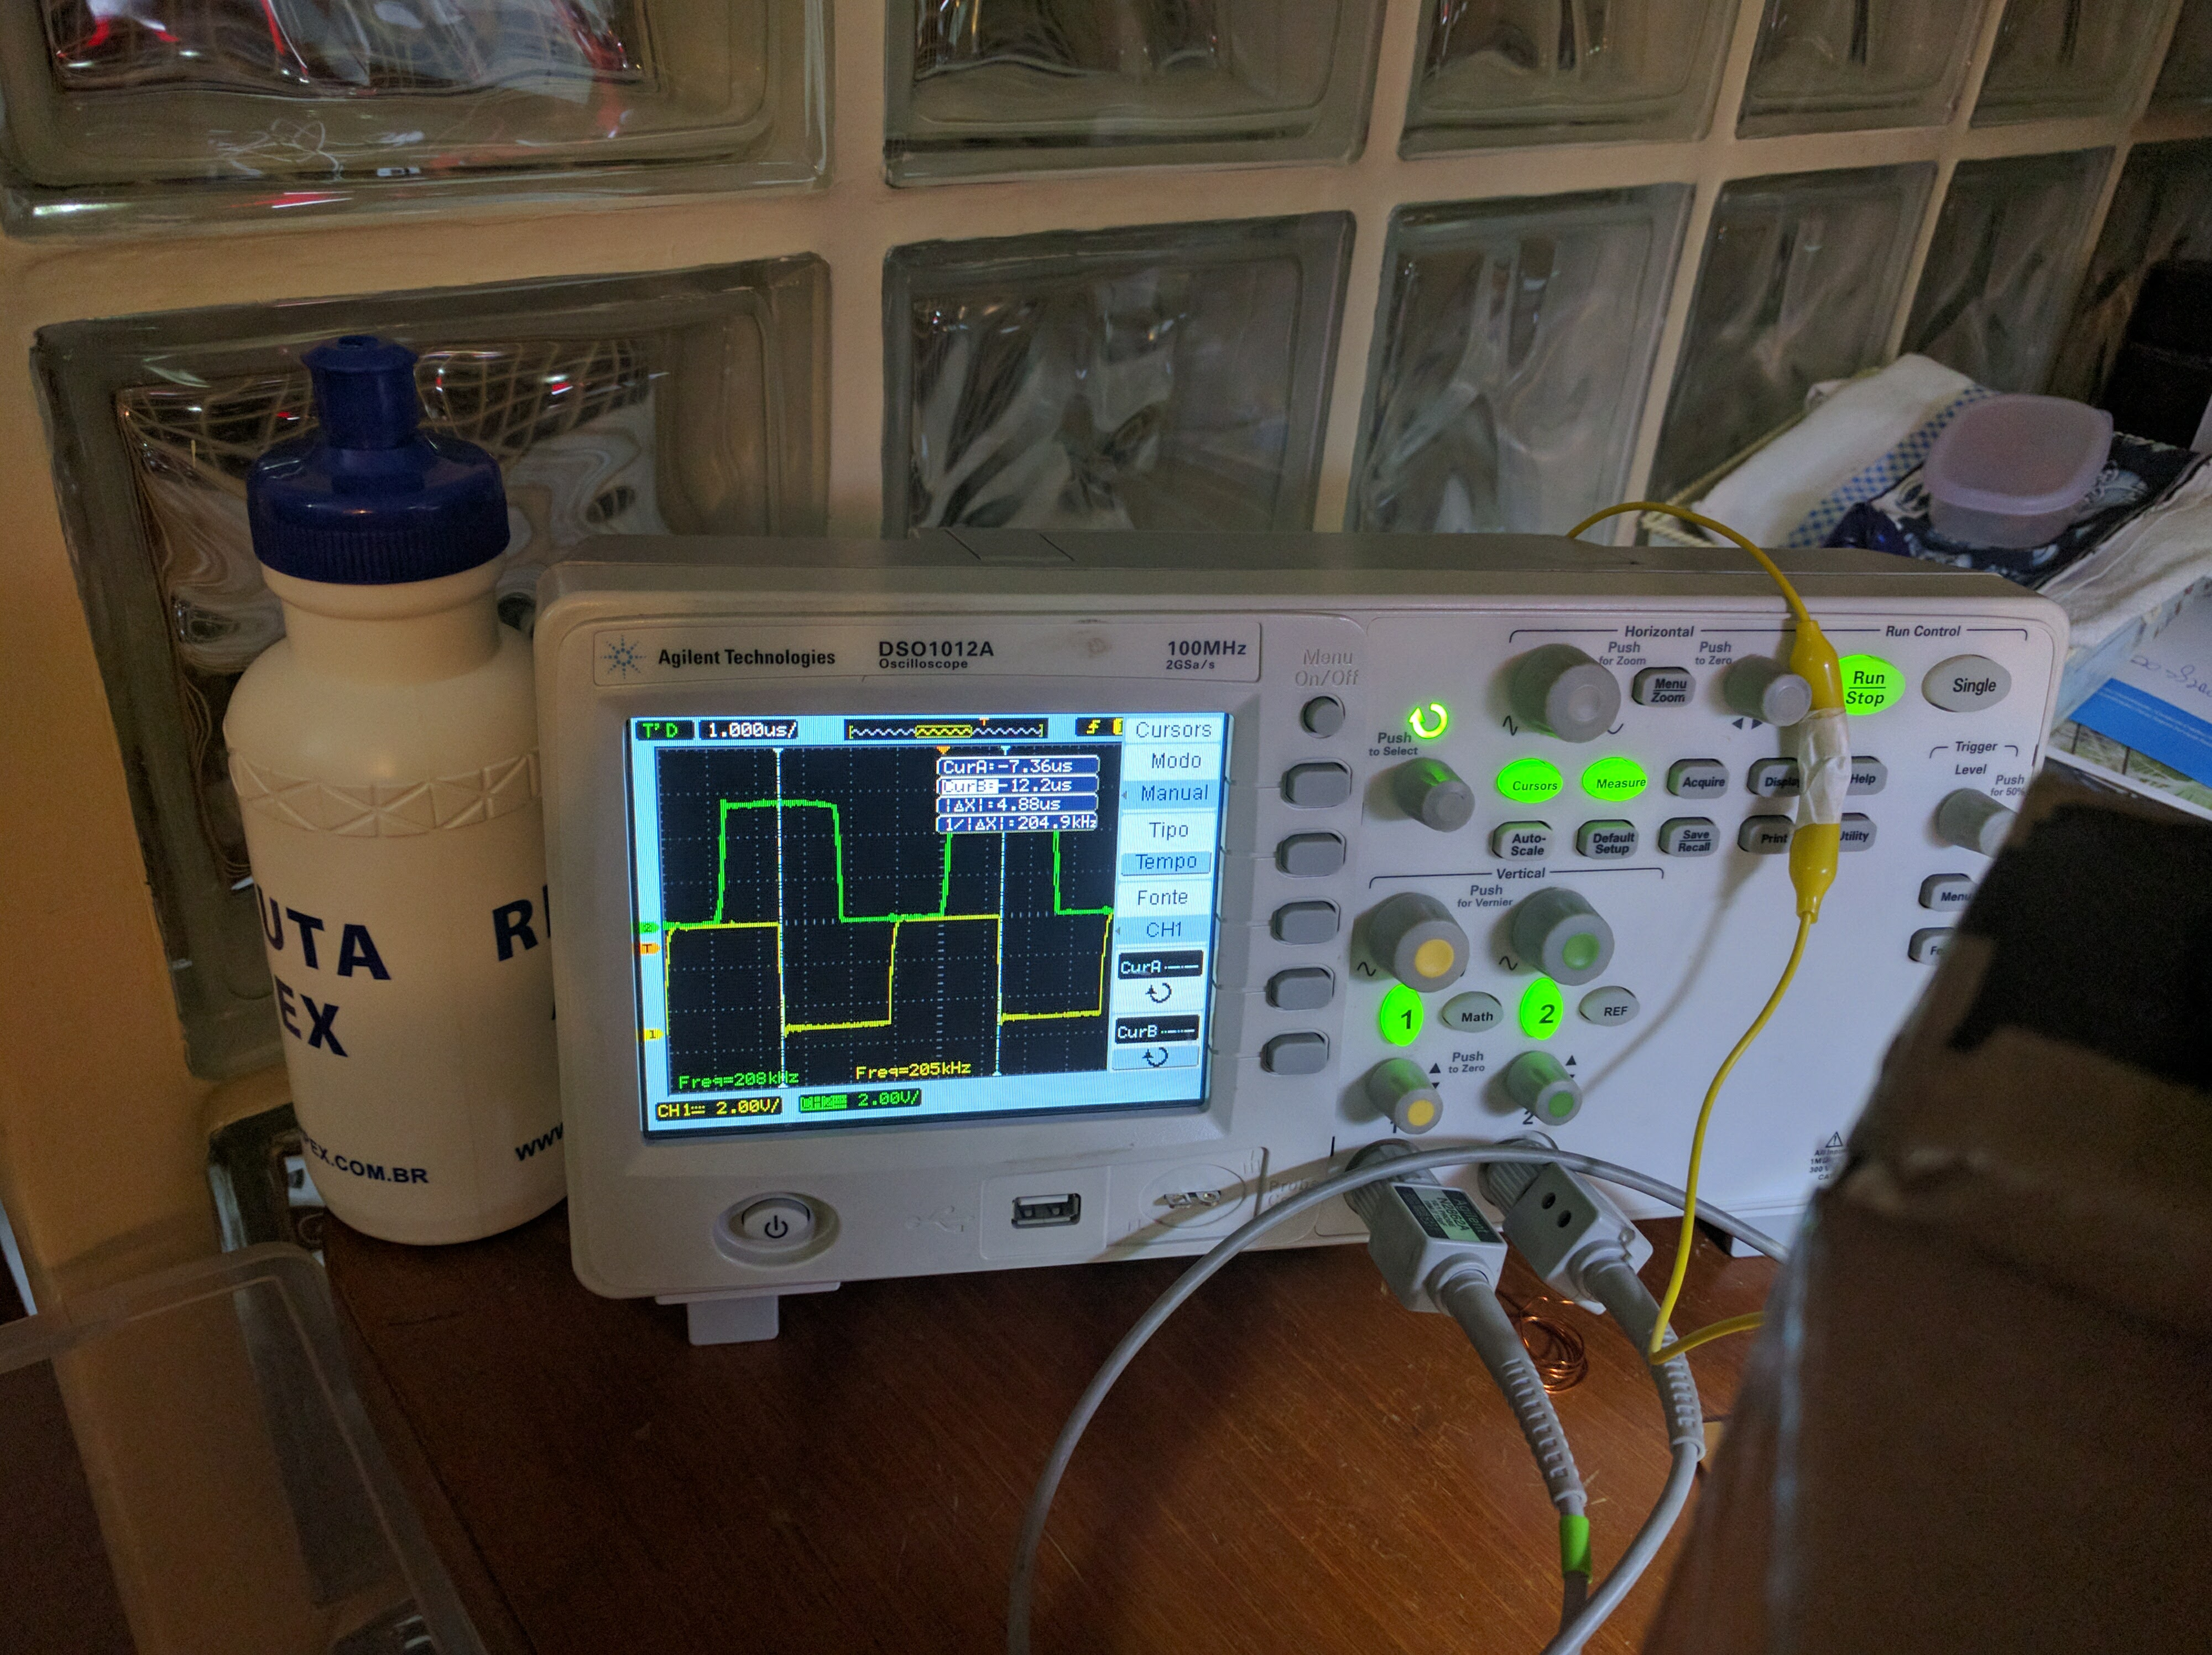
\includegraphics[width=0.7\textwidth, trim={36cm 30cm 60cm 40cm}, clip]{circuits/photos/TXRX_final_fixed.jpg}
		\legend{Fonte: Autores}
	\end{figure}
	
	Em seguida será realizada a integração entre a parte analógica e digital do trabalho.
